\chapter{Experiments And Results}\label{chp:experiments-and-results}
	
	This chapter presents all experiments conducted on the deep learning model that was introduced in chapter~\ref{chp:the_model}.
	The results shown here give useful insights that supplement the work of \cite{wang2017deepvo}.
	
	\section{Dataset Size and Dropout}
		We start by training the proposed model on the KITTI dataset on small subsequences of 25 frames. 
		Initially, the sequences are divided without overlap, that is, each video frame is part of exactly one subsequence.
		In addition, to simulate a dataset with more subsequences, the overlap is set to 20 frames (80\%). 
		This means that for each subsequence there is another one that differs by 5 frames.
		Table~\ref{tbl:kitti-overlap-and-dropout} compares the test error for models trained with and without overlap.
		\begin{table}[tb]
			\small
			\begin{center}
				\begin{tabular}{ccccrrr}
					\toprule
					\multicolumn{3}{c}{\textbf{Experiments}}	&	& \multicolumn{3}{c}{\textbf{Test error}} 		\\
					\cmidrule(lr){1-3} 					\cmidrule(lr){5-7}
					Length 			& Overlap 	& Dropout	&	& Total 	& Rotation	& Translation	\\ 
					\midrule
					25				& 0			& 0			& 	& 19.0293	& 0.4981	& 18.5312		\\ 
					25				& 20		& 0			&	& 16.5471	& 0.3913	& 16.1558		\\ 
					100				& 20		& 0			&	& 529.9459	& 39.8967	& 490.0493		\\ 
					100				& 80		& 0			& 	& 313.1278	& 47.8437	& 265.2841		\\ 
					100 			& 5			& 0.5		&	& 376.7666	& 43.1578	& 333.6088		\\ 
					%$20\rightarrow120$ 	& 5		& 0.5		&	& 303.7696	& 39.4114	& 264.3582		\\
					$20\rightarrow100$ 	& 5		& 0.5		&	& 289.8579 	& 42.0427 	& 247.8152 		\\
					\bottomrule
				\end{tabular}
			\end{center}
			\caption[Experiments on KITTI: Overlap and dropout]
					{Experiments on KITTI: Overlap and dropout. 
					 Shown is the test error on sequence 10 for different overlap and dropout during training.
					 The evaluation on the test set is performed on sequences of the same size as seen during training, and without overlap.
					 In the last row, the sequence length grows by one frame every epoch.
					 Each model was trained with default parameters for 100 epochs, except the last one which was trained for only 80 epochs.
					 \label{tbl:kitti-overlap-and-dropout}}
		\end{table}
		After the same number of epochs, the test error is about 13\% lower for the model trained on overlapping sequences with a decrease of 21\% for rotation and 12\% for translation.
		The same experiment is repeated by training on sequences of 100 frames with overlap 20 vs.\@ overlap 80. 
		% Total error decreases by about 40\%.
		The translation error decreases by almost 46\%, however, the rotation loss increases.
		A similar observation can be made when using dropout on the LSTM output (before the fully-connected layer), as seen in the second last row of table~\ref{tbl:kitti-overlap-and-dropout}.
		
		For the last experiment in table~\ref{tbl:kitti-overlap-and-dropout}, the sequence length grows by an increment of one frame every epoch, starting from 20 frames and stopping at 100 frames after 80 epochs.
		As we can see, this method of training in combination with the dropout gives the best overall loss on the test set.
		A possible explanation for this observation is that the learning process is faster for short sequences because the LSTM requires a less complex memory mapping in order to remember the coordinate transforms from earlier time steps, including the first one.
		A gradual refinement of such a mapping may be less challenging for the optimization as opposed to learning it directly from long sequences.
		
		Although the numbers in the table can be used to compare the different experiments, they are not very insightful by themselves.
		From the sum of squared differences alone, it is not possible to understand how the error behaves across the sequence.
		For better visualization, we can compute the error at regular distance intervals along the estimated path.
		Figure~\ref{fig:kitti-avg-rotation-translation-error-vs-path-distance} shows translation and rotation errors for path distance on subsequences of the KITTI sequence 10.
		\begin{figure}[t]
			\centering
			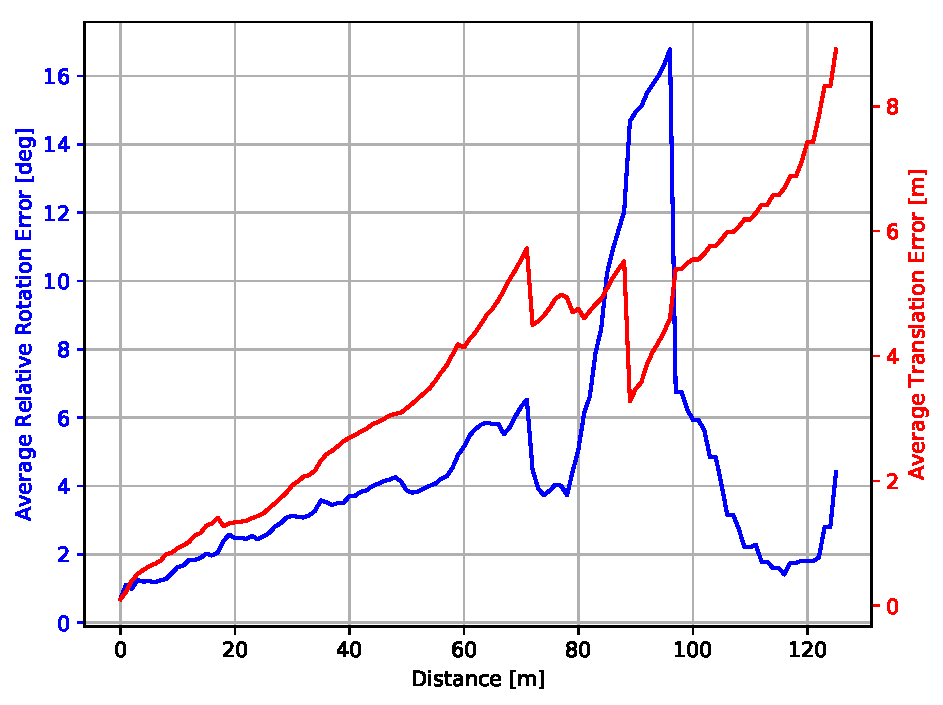
\includegraphics[width=0.7\linewidth]{Python-Plots/deepvo-KITTI/relative-rotation-and-translation-error-along-path-overlap80}
			\caption[Experiments on KITTI: Average rotation- and translation error vs.\@ path distance]
					{Experiments on KITTI: Average rotation- and translation error vs.\@ path distance.
					 The relative rotation- and translation error is evaluated at equal intervals along the subsequences of KITTI sequence 10.
					 The errors at the same distance are averaged over all sequences of that length.
					 \label{fig:kitti-avg-rotation-translation-error-vs-path-distance}}
		\end{figure}
		The relative rotation error is the angle of rotation around the axis corresponding to the relative rotation between estimated- and ground truth pose.
		
		\paragraph{Discussion}
		From these experiments, we can conclude that sequence overlap and dropout have a positive impact on the generalization of translation estimates.
		Especially when training data is scarce, the overlap method can be utilized to artificially increase the dataset and reduce the error on the test data.
		
	\section{The Problem on Long Sequences}
		In the experiments before, the model was always tested on subsequences with the same length as during training.
		However, in a real-world application, we would like to test the model on sequences with an arbitrary number of frames, and potentially the test sequences are much longer than the ones seen during training.
		Table~\ref{tbl:kitti-testing-on-longer-sequences} shows an experiment where the sequence length between training set and test set changes.
		The problem: The model trained on sequences with 25 frames does not generalize to sequences of 100 frames.
		This is a very undesired result, after all, the recurrent part of the network was designed with the intention to handle arbitrary input sizes.
		From the results in table~\ref{tbl:kitti-testing-on-longer-sequences} it appears that the network is able to memorize the sequence length and therefore overfits to the specific length it is trained on.
		The attempt to counteract this behavior with sequences of random size failed.
		The network would still overfit to the average length of sequences seen during training.
		Figure~\ref{fig:kitti-testing-on-longer-sequences} visualizes the camera path on a test sequence of 100 frames.
		\begin{figure}
			\centering
			\begin{subfigure}[b]{0.5\linewidth}
				\centering
				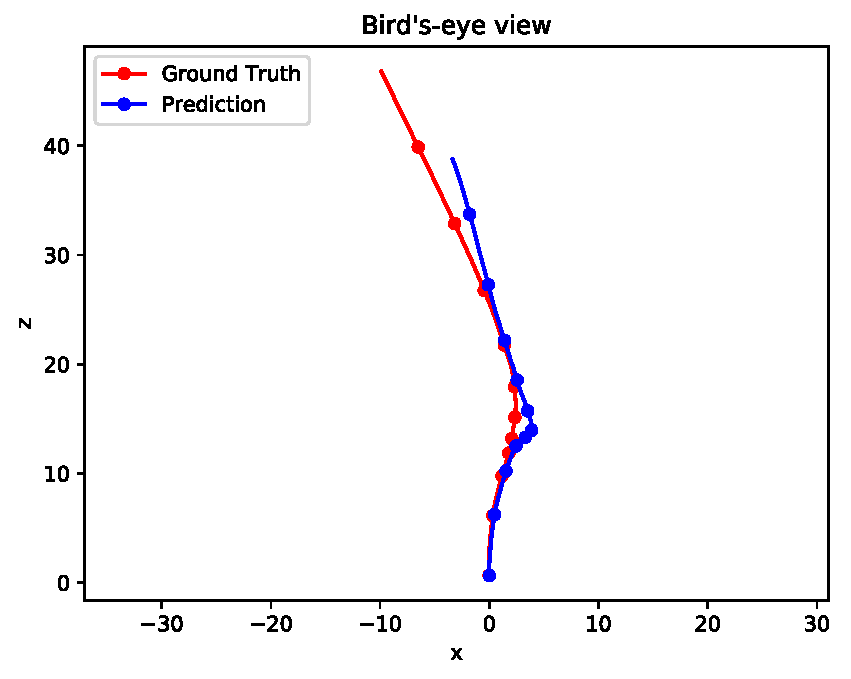
\includegraphics[width=\linewidth]{Experiments/trained-on-25-frames}
				\caption{
					\label{fig:0}
				}
			\end{subfigure}%
			\begin{subfigure}[b]{0.5\linewidth}
				\centering
				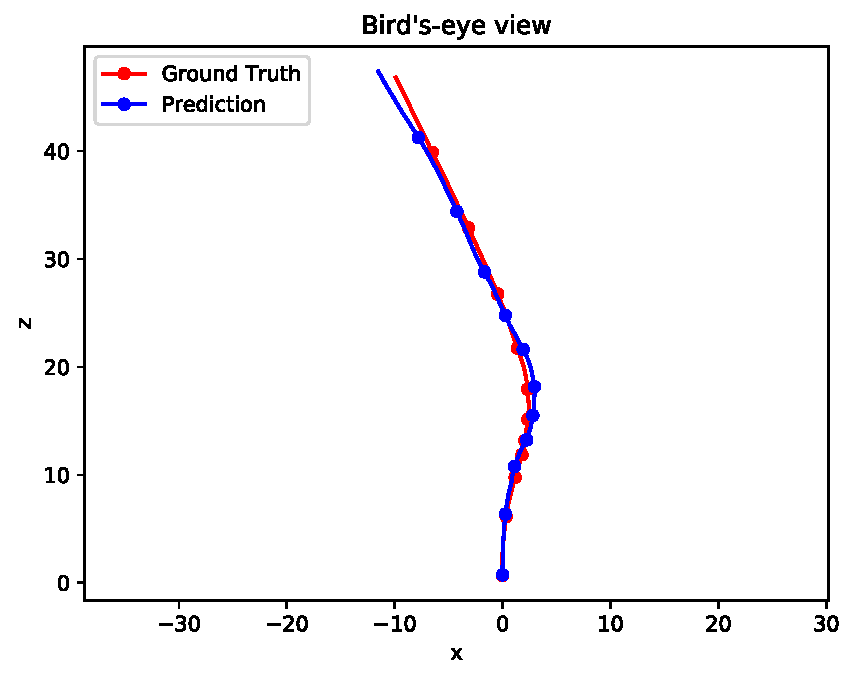
\includegraphics[width=\linewidth]{Experiments/trained-on-100-frames}
				\caption{
					\label{fig:1}
				}
			\end{subfigure}%
			\caption[Training and testing on different sequence length]
					{Training and testing on different sequence length. 
					 Two models tested on a KITTI subsequence of 100 frames when trained on sequences of (a) 25 frames and (b) 100 frames. 
					 The markers in the plot are shown every ten frames.
					 The scale of the axes is in meters.
					 \label{fig:kitti-testing-on-longer-sequences}}
		\end{figure}
		\begin{table}[tb]
			\small
			\begin{center}
				\begin{tabular}{cccrrr}
					\toprule
					\multicolumn{2}{c}{\textbf{\#Frames}}	&	& \multicolumn{3}{c}{\textbf{Test error}} \\ 
					\cmidrule(lr){1-2} 									\cmidrule(lr){4-6}
					Training 		& Test 			&	& Total 	& Rotation	& Translation	\\ 
					\midrule
					25				& 25			&	& 16.5471	& 0.3913	& 16.1558		\\
					25				& 100			&	& 1060.7528	& 37.6196	& 1023.1332		\\
					100				& 100			&	& 529.9459	& 39.8967	& 490.0493		\\ 
					\bottomrule
				\end{tabular}
			\end{center}
			\caption[Experiments on KITTI: Testing on longer sequences]
					{Experiments on KITTI: Testing on longer sequences. 
					 When testing on sequences with more frames, the error becomes extremely high compared to the model trained on 100 frames.
					 \label{tbl:kitti-testing-on-longer-sequences}}
		\end{table}
		One can observe that the estimated path quickly diverges after 25 frames.
		However, when trained on sequences with 100 frames, the estimation is more accurate.
		
		\paragraph{Discussion}
		The experiments in this section reveal a serious problem.
		One of the main purposes of the LSTM is to handle arbitrary input length, and yet, in the scenario we have so far it is not able to do so.
		In the general application of VO, it is not realistic to assume a maximum length for a video and to train the model only for that length.
		
		
	\section{Training with Incremental Poses}
		One potential reason for why the model is overfitting to a certain length could be semantic difference between input and output.
		Since input at each time step is a pair of consecutive images in the video, the observed motion (by the LSTM) is relative to the current time step.
		On the other hand, the output pose is forced to be in the global coordinate system given by the very first video frame.
		This difference could potentially cause confusion and lead to the overfitting problem.
		
		To address the issue, we convert the ground truth poses to incremental poses using the formula from equation~\ref{eq:relative_rotation_conversion_general} by setting $j = i - 1$.
		Table~\ref{tbl:kitti-incremental-pose-and-lstm-removal} shows the results of training with incremental pose.
		At test time, the output poses are converted back into the global coordinate system for evaluating the loss on the test set.
		This allows for a direct comparison with the previous results from table~\ref{tbl:kitti-testing-on-longer-sequences}.
		\begin{table}[tb]
			\small
			\begin{center}
				\begin{tabular}{ccccrrr}
					\toprule
					\multicolumn{4}{c}{\textbf{Experiments}}		& \multicolumn{3}{c}{\textbf{Test error}} 		\\
					\cmidrule(lr){1-4} 	\cmidrule(lr){5-7}
					\multicolumn{2}{c}{Length} & Dropout &	& Total & Rotation & Translation	\\ 
					Training & Test & & & & & \\
					\midrule
					25 & 25		& 0				& 	& 22.0498	& 0.5642	& 21.4856 		\\ 
					25 & 25		& 0.5			& 	& 21.0171	& 0.4957	& 20.5214		\\ 
					%25 & 25		& 0			& \xmark 	& 	& 22.4305	& 0.5121	& 21.9184		\\ 
					\midrule
					25 & 100	& 0			 	& 	& 335.5754	& 16.5476	& 319.0277 		\\ 
					25 & 100	& 0.5		 	& 	& 301.5090	& 22.9736	& 278.5354		\\ 
					%25 & 100	& 0			& \xmark 	& 	& 378.8834	& 48.4604	& 330.4230 		\\ 
					\bottomrule
				\end{tabular}
			\end{center}
			\caption[Experiments on KITTI: Training with incremental poses]
					{Experiments on KITTI: Training with incremental poses.
					 Three variants are tested: LSTM, LSTM with dropout layer, and LSTM replaced with fully-connected layer.
					 Shown is the loss on the test set with incremental poses converted to global poses.
					 \label{tbl:kitti-incremental-pose-and-lstm-removal}}
		\end{table}
		From these results we can see that the error is significantly lower when testing on long sequences.
		Since the only difference in the experiments is the format of the pose, it can be concluded that training with incremental pose is the preferred way.
		In the paper of \cite{wang2017deepvo}, it is never explicitly stated which coordinate system is used.
		The results in this thesis suggest that \citeauthor{wang2017deepvo} have also used incremental poses in their experiments.
		Qualitative results for motion estimation on the KITTI test data are presented in figure~\ref{fig:kitti-qualitative-results-images-and-estimation}.
		They show how the system handles scenes with moving objects, sharp turns and change of speed.
		
		The new approach of training the network with incremental poses raises an important question.
		What exactly is the contribution of the LSTM?
		Since the pose is not global anymore, the LSTM is not forced to keep track of the accumulation of pose changes from the past frames.
		To investigate this question, we conduct an experiment where the LSTM is replaced with a fully-connected layer followed by a ReLU.
		The previous affine output layer is kept, making it a total of two affine layers that regress the pose from the CNN features.
		This eliminates the recurrence from the network, and all pose estimations are performed solely on consecutive frames.
		Each output is independent of the previous inputs, therefore it is simply a feedforward network.
		For these experiments, the VIPER dataset is used instead of KITTI.
		The table~\ref{tbl:viper-effect-of-replacing-LSTM} compares the non-recurrent model with two recurrent models, one with a hidden size $d = 1000$ and one with $d = 500$.
		Both recurrent versions operate only with one LSTM layer as opposed to two as before.
		This should make for a fairer comparison.
		Alternatively, one could have chosen to insert two affine layers instead of one and compare with a two-layer LSTM.
		The test errors in table~\ref{tbl:viper-effect-of-replacing-LSTM} show that the recurrent models perform better for pose, but worse for translation compared to the non-recurrent version.
		Additionally, in figure~\ref{fig:avg-rotation-error-VIPER-LSTM-no-LSTM} we observe that the rotation error at long distances is significantly higher for the non-recurrent model.
		
		\begin{figure}
			\centering
			\begin{subfigure}[b]{0.5\linewidth}
				\centering
				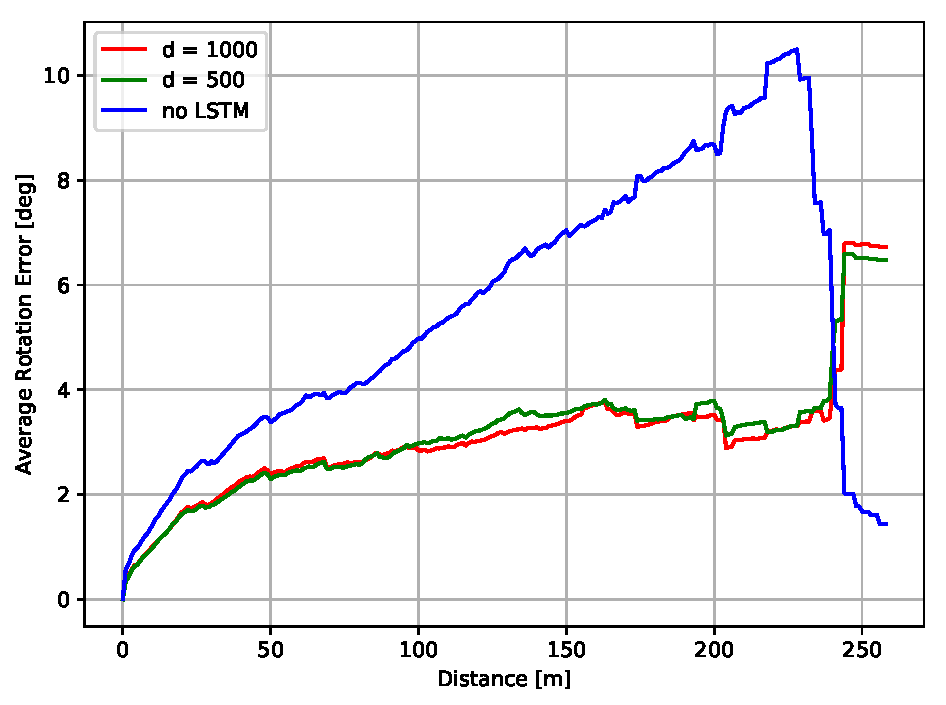
\includegraphics[width=\linewidth]{Python-Plots/deepvo-VIPER/rotation-error-per-meter-comparison-LSTM-No-LSTM-v2}
				\caption{
					Rotation
					\label{fig:avg-rotation-error-VIPER-LSTM-no-LSTM}
				}
			\end{subfigure}%
			\begin{subfigure}[b]{0.5\linewidth}
				\centering
				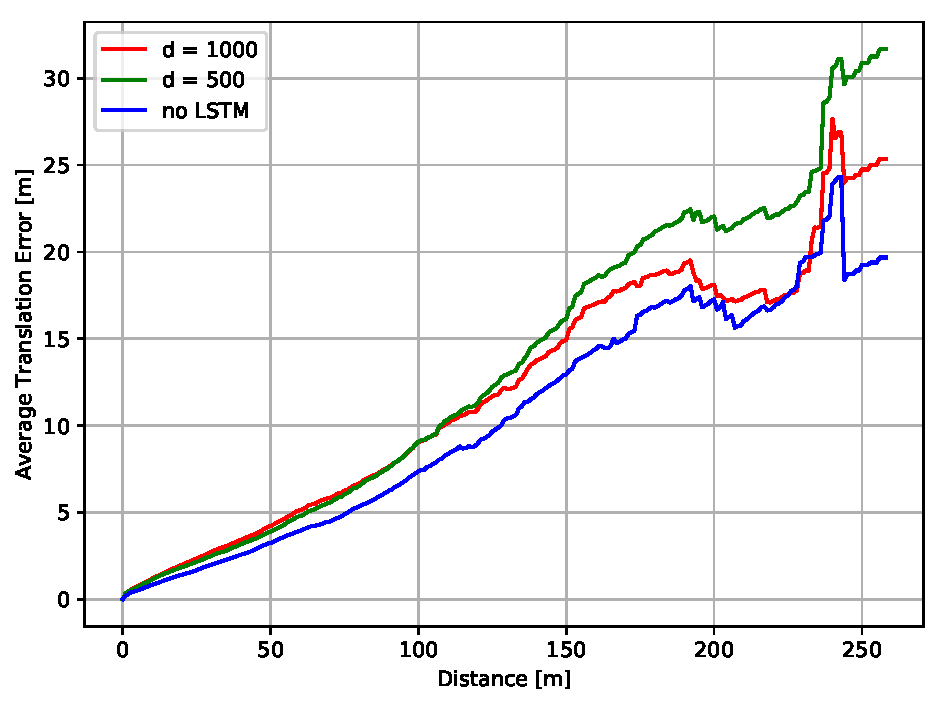
\includegraphics[width=\linewidth]{Python-Plots/deepvo-VIPER/translation-error-per-meter-comparison-LSTM-No-LSTM-v2}
				\caption{
					Translation
					\label{fig:avg-translation-error-VIPER-LSTM-no-LSTM}
				}
			\end{subfigure}%
			\caption[Experiments on VIPER: The effect of replacing the LSTM]
					{Comparison of the recurrent and non-recurrent models on the VIPER test dataset.
					 The recurrent versions have an overall lower rotation error, but they are worse translation error compared to the non-recurrent model.
					 \label{fig:viper-effect-of-replacing-LSTM}}
		\end{figure}
		
		\begin{table}[tb]
			\small
			\begin{center}
				\begin{tabular}{cccrrrr}
					\toprule
					\multicolumn{2}{c}{\textbf{Experiments}} & & \multicolumn{2}{c}{\textbf{Incremental Pose}} & \multicolumn{2}{c}{\textbf{Global Pose}} \\
					LSTM 	& Hidden size 		& 	& Rotation 	& Translation & Rotation & Translation \\
					\midrule
					\xmark	& -- 				&	& 0.2162	& \underline{7.3836}	& 6.7071	& \underline{241.1611}		\\
					\cmark	& 1000				& 	& 0.1625	&	7.4642 	& 4.8312&	285.5663		\\
					\cmark 	& 500				& 	&\underline{0.1581}	& 7.5345 	& \underline{4.3250}&	286.7348	 \\
					\bottomrule
				\end{tabular}
			\end{center}
			\caption[Experiments on VIPER: The effect of replacing the LSTM]
					{Experiments on VIPER: The effect of replacing the LSTM.
					 All models are trained for 100 epochs and tested on sequences of 100 frames with both incremental- and global pose.
					 The recurrent versions perform best in terms of rotation error, whereas the non-recurrent version has lower translation error.
					 \label{tbl:viper-effect-of-replacing-LSTM}}
		\end{table}
		
		\paragraph{Discussion}
		In this second set of experiments, we have addressed the issue where the LSTM would overfit to a certain number of frames seen during training.
		When forced to output incremental poses, the model is able to estimate motion from videos of arbitrary sizes.
		However, it is still unclear if and to what amount the LSTM uses the hidden state that encodes the past.
		In fact, as we have shown, a feedforward network (without recurrence) is able to outperform the LSTM in positional error.
		Based on these observations, one might speculate that the recurrent connection hurts the performance.
		But this is not a very plausible, because during the optimization process the LSTM would learn to ignore the hidden state by setting the parameters of the cell gates accordingly, if this minimizes the loss.
		It is possible that the loss function in equation~\ref{eq:euler_pose_loss_function_t}, a balance between euclidean error of translation and rotation, is not well-suited for VO.
		The balance factor $\beta$ is chosen manually with a simple heuristic based on the fraction between expected translation- and rotation error.
		In a way, the balance factor tells the optimization algorithm how important the accuracy for rotation is compared to the position.
		It is certainly possible that the choice of $\beta$ has a significant impact on the networks ability to properly separate rotation and translation from the input.
		As the scale of the motion between frames heavily depends on the dataset, it is not viable to systematically search through values for $\beta$ for different datasets.
		A way to eliminate the balance factor is left for future work.
		
	\section{Pose Representation and State Transfer}
		For all experiments so far, the hidden state $\vectr{h}_t$ of the LSTM is reset (re-initialized as zero) before the next video sample is fed because it is assumed that the videos in the dataset are shuffled.
		A state transfer from one video to the other would not make sense if the two are different.
		Also, in the case of global pose where each pose is relative to the first frame in the sequence, the hidden state can not be transfered as the coordinate system would change from one video to the next.
		However, when training on incremental motions between pairs of frames, it is possible to carry the state from one video to the other when the subsequences are kept in the same order as they occur in the original full video.
		In this case, backpropagation in time is still only performed over the frames in the subsequence, and not to the very beginning.
		
		Table~\ref{tbl:viper-state-reset-vs-keep} compares the test errors of the two forms of training with hidden state.
		The experiment shows that resetting the state results in lower test errors for both rotation and translation.
		\begin{table}[tb]
			\small
			\begin{center}
				\begin{tabular}{lcrrrr}
					\toprule
					\textbf{Hidden state} & & \multicolumn{2}{c}{\textbf{Incremental Pose}} & \multicolumn{2}{c}{\textbf{Global Pose}} \\
					& & Rotation & Translation & Rotation & Translation \\
					\midrule
					Keep		&			& 0.3097	& 8.5461	& 12.7551	& 426.7877		\\
					Reset 		& 			& 0.2319	& 5.7220	& 9.8600	& 262.7984		\\ 
					\bottomrule
				\end{tabular}
			\end{center}
			\caption[Experiments on VIPER: State persistence vs.\@ reset]
					{Experiments on VIPER: State persistence vs.\@ reset.
					 Both models are identical and trained with with the same hyperparameters with the only difference being how the hidden state is handled.
					 \label{tbl:viper-state-reset-vs-keep}}
		\end{table}
		Additionally, as shown in figure~\ref{fig:viper-convergence-speed-state-reset-vs-keep}, the convergence speed on the validation set is greater for the method that resets the state.
		The training error converges with the same speed for both methods. 
		\begin{figure}[t]
			\centering
			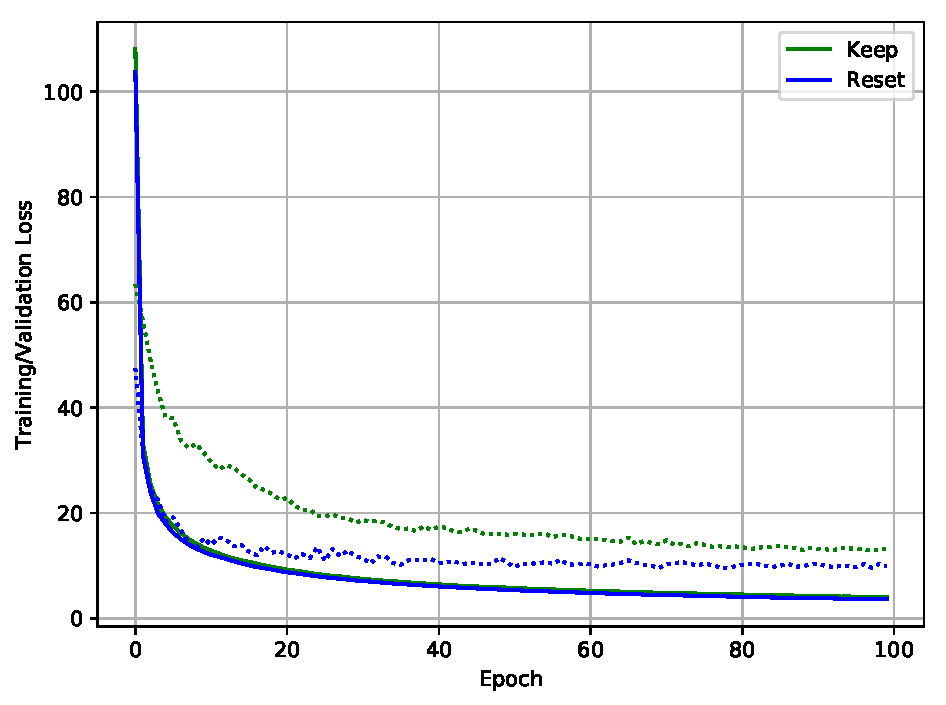
\includegraphics[width=0.7\linewidth]{Python-Plots/deepvo-VIPER/convergence-speed-keep-vs-reset}
			\caption[Convergence speed comparison: State persistence vs.\@ reset]
					{Convergence speed comparison: State persistence vs.\@ reset.
					 Two identical models are trained on the VIPER dataset.
					 In one model (blue), the recurrent state is reset after each video sample.
					 In the other case (green), the hidden state is carried over for the next video.
					 The dotted lines show the validation error.
					 \label{fig:viper-convergence-speed-state-reset-vs-keep}}
		\end{figure}
		This experiment gives another indication that the recurrent connection might influence the learning process in a negative way.
		But the question remains why the optimization does not adjust the weights accordingly such that the hidden state vector is simply ignored.
		
		Further experiments show that it is unlikely that the pose representation is the problem.
		In figure~\ref{fig:viper-euler-vs-quat-vs-hidden-state-keep-or-reset}, combinations of state management and pose representations are compared in terms of rotation- and translation error on VIPER.
		\begin{figure}
			\centering
			\begin{subfigure}[b]{0.5\linewidth}
				\centering
				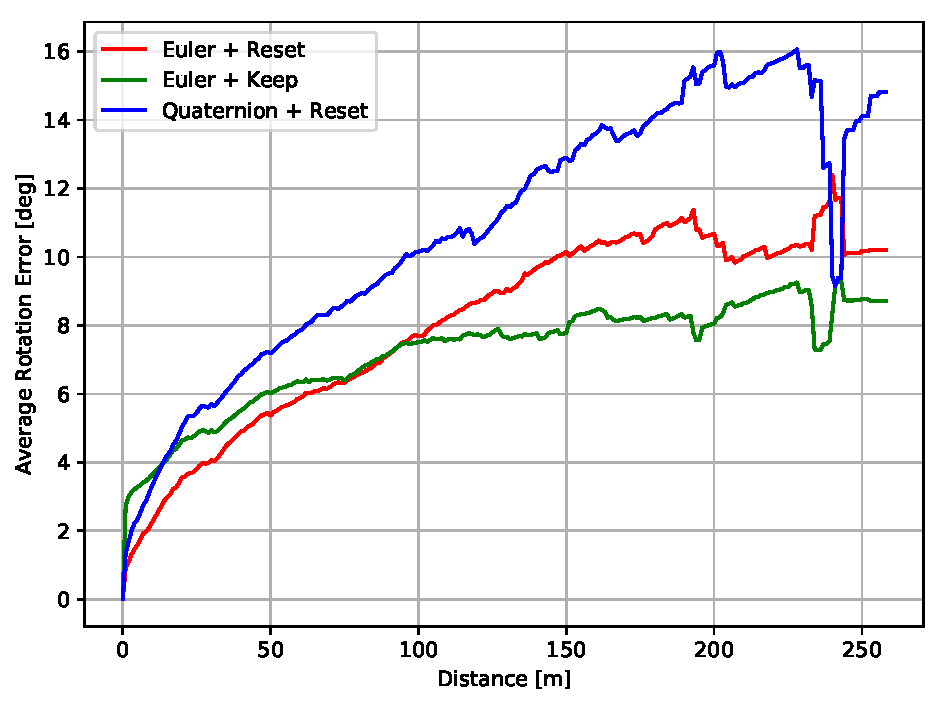
\includegraphics[width=\linewidth]{Python-Plots/deepvo-VIPER/rotation-comparison-Euler-Quaternion-Reset-or-Keep-Hidden}
				\caption{Rotation}
			\end{subfigure}%
			\begin{subfigure}[b]{0.5\linewidth}
				\centering
				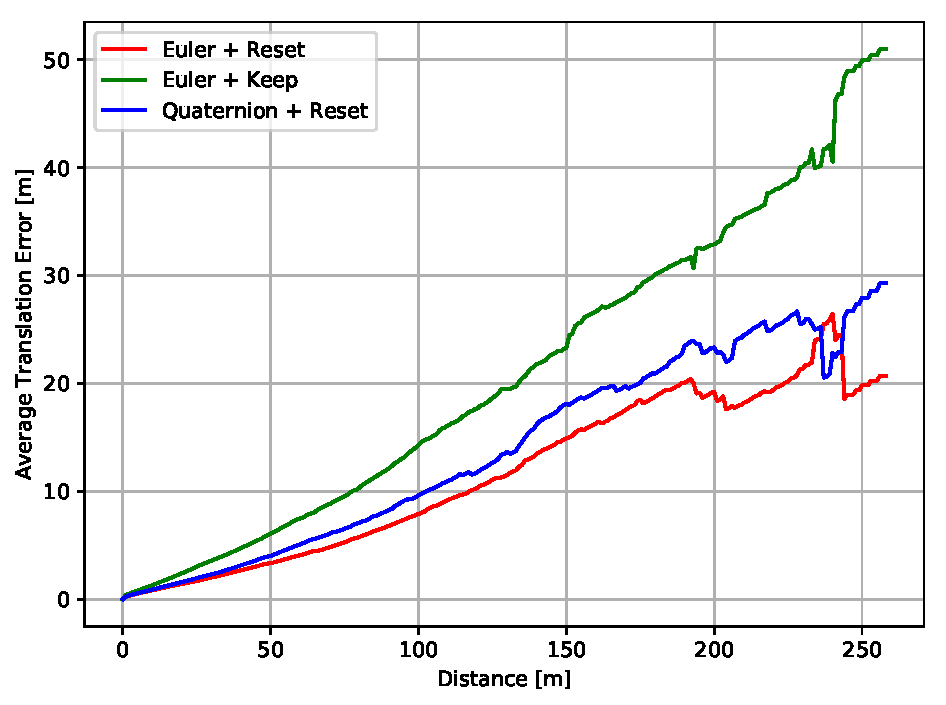
\includegraphics[width=\linewidth]{Python-Plots/deepvo-VIPER/translation-comparison-Euler-Quaternion-Reset-or-Keep-Hidden}
				\caption{Translation}
			\end{subfigure}%
			\caption[Experiments on VIPER: Euler vs.\@ quaternion vs.\@ hidden state transfer]
					{Experiments on VIPER: Euler vs.\@ quaternion vs.\@ hidden state transfer.
					 In all experiments, the model was trained for 50 epochs on videos of 100 frames.
					 No dropout is applied.
					 \label{fig:viper-euler-vs-quat-vs-hidden-state-keep-or-reset}}
		\end{figure}
		For the model where the rotations are represented by unit quaternions, the loss from equation~\ref{eq:quaternion_pose_loss_function_t} is used.
		In order to compare all versions, the rotations are converted to Euler angles at test time and evaluated using the Euclidean loss as before (eq.\@~\ref{eq:euler_pose_loss_function_t}).
		From these results we can make two main observations.
		First, training with Euler angles (red) results in better performance compared to training with quaternions (blue), both for rotational- and translational error.
		Second, for the model trained with persistent hidden state, the rotation error is the lowest, but the translation error is highest among the others.
		Therefore, when comparing all three, there is no clear winner.
		
		\paragraph{Discussion}
		Why do Euler angles work better than quaternions?
		A possible explanation is that the complexity of the mapping for incremental pose changes is higher for the model where quaternions are used.
		Small rotational motions in the input result in small Euler angles, and on the other hand, large rotational motions imply larger Euler angles.
		The relationship between input rotation and output quaternion is more complex.
		As the unit-quaternion is parameterized by 
		$
			\vectr{q} = 
			\cos\left(\tfrac{\theta}{2}\right) + 
			\sin\left(\tfrac{\theta}{2}\right) \left(a_1 \vectr{i} + a_2 \vectr{j} + a_3 \vectr{k}\right),
		$
		the LSTM is forced to regress the four components that contain sine and cosine.
		A two-layer LSTM with sigmoid and hyperbolic tangent activation functions (eq.\@ \ref{eq:Vanilla-LSTM-Definition}) might not be powerful enough to approximate the mapping of angle and axis in combination with the cosine- and sine components.
		Further investigation on this manner is a possibility for future work.
		
	\section{Evaluation on the GTA V Dataset}
		In contrast to the VIPER dataset where most videos are captured from a driving vehicle, in our dataset all motions are captured on foot.
		Additionally, the frame rate of 30 fps in GTA V is twice as high as in VIPER.
		The scale of motion between consecutive frames in the videos is compared in table~\ref{tbl:viper-gta-comparison-inter-frame-motion}.
		\begin{table}[tb]
			\small
			\begin{center}
				\begin{tabular}{lcrrcrr}
					\toprule
					\textbf{Dataset} 		& 	& \multicolumn{2}{c}{\textbf{Rotation [deg]}} 		& & \multicolumn{2}{c}{\textbf{Distance [m]}} 		\\
									& 	& Average 		& Maximum			&	& Average 		& Maximum					\\
					\midrule
					GTA V 30 fps 	& 	&  0.9488	& 31.0659 		&	& 0.1286 	& 0.5440 				\\
					GTA V 15 fps*	& 	&  1.8976	& 62.1318		& 	& 0.2572	& 1.0880				\\
					VIPER 15 fps	&   & 0.5284	& 15.6798 		& 	& 0.6792	& 6.6327				\\
					\bottomrule
				\end{tabular}
			\end{center}
			\caption[Inter-frame motion comparison between the VIPER and GTA V datasets]
					{Inter-frame motion comparison between the VIPER and GTA V datasets.
					 The table shows the relative rotation angle and traveled distance between consecutive frames on the test set.
					 Since the GTA V videos are captured with twice the frame rate as VIPER, the numbers are multiplied by two and shown in the second row (*) for direct comparison with VIPER. 
					 \label{tbl:viper-gta-comparison-inter-frame-motion}}
			%		GTA
			%		Statistics for training set:
			%		Rotation angle between consecutive frames (AVG / MIN / MAX): 0.9147 / 0.0000 / 175.0265 degrees
			%		Distance travelled between consecutive frames (AVG / MIN / MAX): 0.1298 / 0.0000 / 0.6191 meters
			
			%		VIPER
			%		Statistics for training set:
			%		Rotation angle between consecutive frames (AVG / MIN / MAX): 0.5992 / 0.0000 / 23.1485 degrees
			%		Distance travelled between consecutive frames (AVG / MIN / MAX): 0.6938 / 0.0000 / 8.0416 meters
		\end{table}
		In VIPER, the camera is usually pointing in the forward driving direction, whereas in \mbox{GTA V} the camera is turned freely in all directions while walking and exploring the video game world.
		The average rotation angle in VIPER is lower compared to GTA V, since there are only a few rapid rotation movements in short periods of time.
		Although the traveled distance per frame in VIPER is longer, the freedom of motion in a car is limited as it can move forward or backward, but not to the side.
		Some qualitative results for motion estimation trained on VIPER are shown in figure~\ref{fig:viper-qualitative-results-images-and-estimation}.
		The Euler angle representation for pose is used in this setting.
		Even though the data is synthetic, the images in the figure show that the system is exposed to realistic and challenging scenarios, where multiple object (like cars) interact with the scene in different lighting and weather conditions.
		
		The higher diversity of motion in GTA V makes the dataset more challenging for VO compared to VIPER and even KITTI.
		Qualitative results of the proposed VO applied to GTA V is shown in figures~\ref{fig:gtav-qualitative-results-images-and-translation} and~\ref{fig:gtav-qualitative-results-translation}.
		In this case, the quaternion pose representation together with the loss from equation~\ref{eq:quaternion_pose_loss_function_t} was used for training.
		We observe that the estimations for the translation are not very impressive.
		The system can not handle motions with sharp turns (fig.\@~\ref{fig:gtav-qualitative-sharp-turn}) or motions in wide open areas where structures like houses and mountains are far away.
		
		
		\begin{figure}[h]
			\centering
			\begin{subfigure}[t]{\linewidth}
				\centering
				\raisebox{8mm}{
					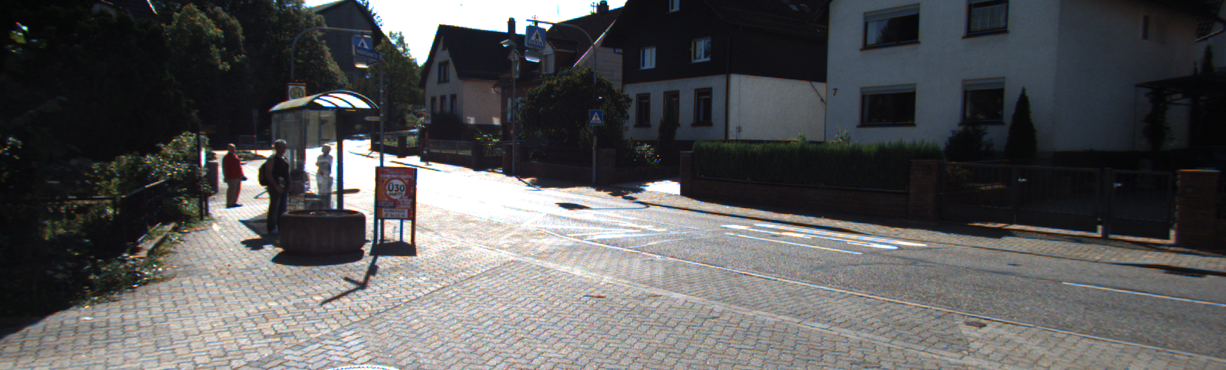
\includegraphics[width=0.5\linewidth, trim={5cm 0 9cm 0}, clip]{Experiments/kitti/000607}
				}
				\includegraphics[width=0.45\linewidth]{Experiments/kitti/pdf/bird-0007}
				\caption{
					Change of speed at intersection
					\label{fig:kitti-qualitative-speed-change}
				}
			\end{subfigure}%
			\\
			\begin{subfigure}[b]{\linewidth}
				\centering
				\raisebox{8mm}{
					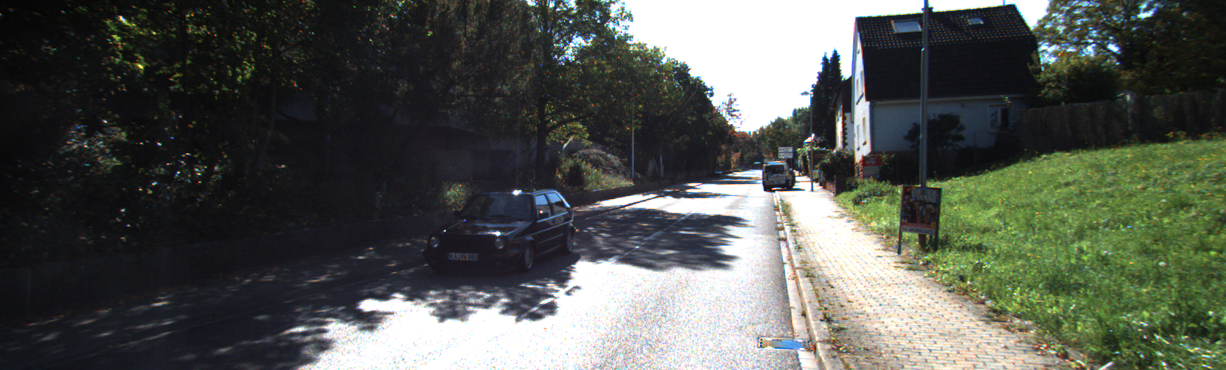
\includegraphics[width=0.5\linewidth, trim={5cm 0 9cm 0}, clip]{Experiments/kitti/000728}
				}
				\includegraphics[width=0.45\linewidth]{Experiments/kitti/pdf/bird-0008}
				\caption{
					Dynamic motion from traffic
					\label{fig:kitti-qualitative-traffic-1}
				}
			\end{subfigure}%
			\\
			\begin{subfigure}[b]{\linewidth}
				\centering
				\raisebox{8mm}{
					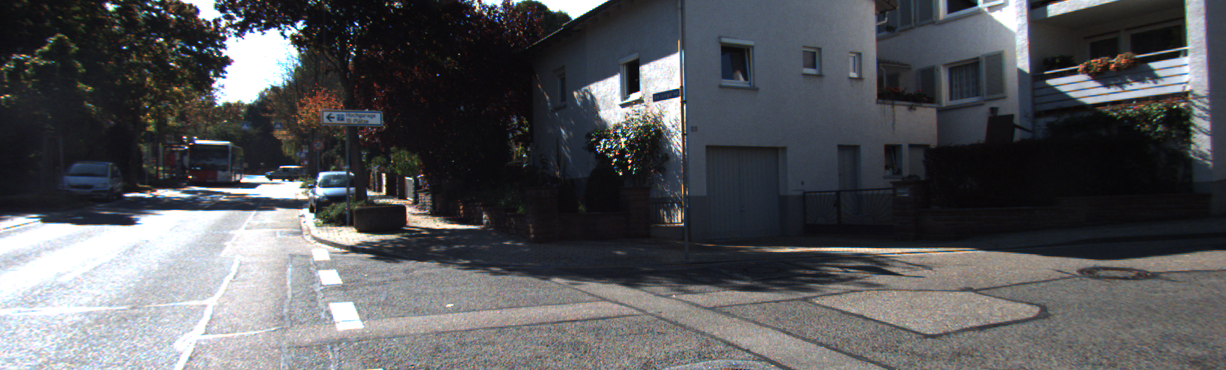
\includegraphics[width=0.5\linewidth, trim={5cm 0 9cm 0}, clip]{Experiments/kitti/000858}
				}
				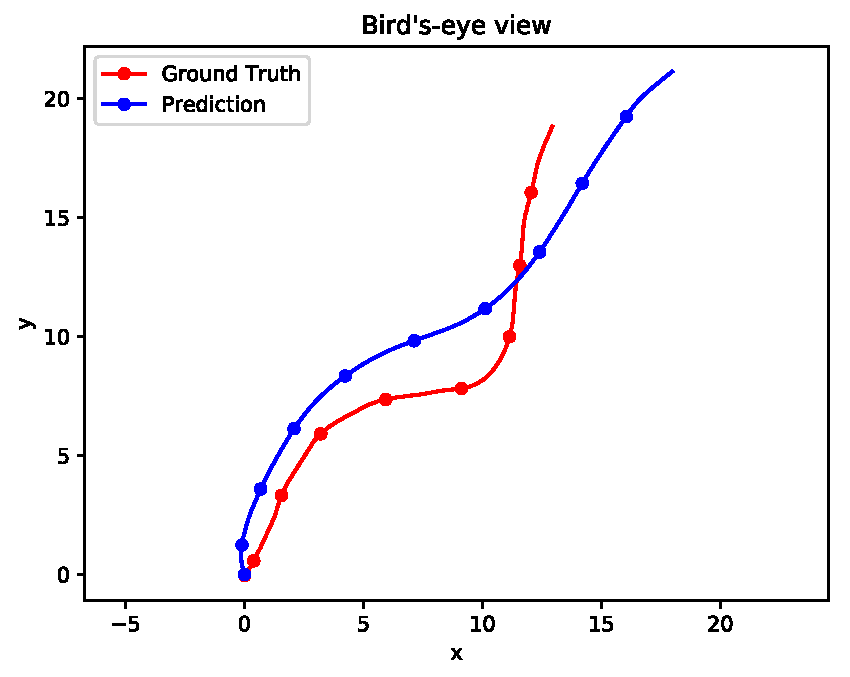
\includegraphics[width=0.45\linewidth]{Experiments/kitti/pdf/bird-0009}
				\caption{
					Sharp right-hand bend
					\label{fig:kitti-qualitative-sharp-turn}
				}
			\end{subfigure}%
			\\
			\begin{subfigure}[b]{\linewidth}
				\centering
				\raisebox{8mm}{
					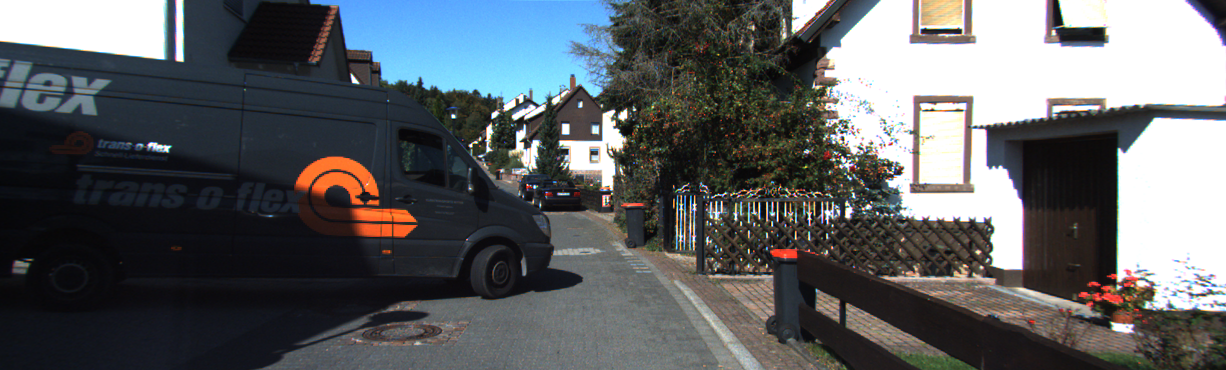
\includegraphics[width=0.5\linewidth, trim={5cm 0 9cm 0}, clip]{Experiments/kitti/000992}
				}				\includegraphics[width=0.45\linewidth]{Experiments/kitti/pdf/bird-0010}
				\caption{
					Change of speed and scene motion in close proximity
					\label{fig:kitti-qualitative-truck-close-up-stop}
				}
			\end{subfigure}%
			\caption[Qualitative results for motion estimation on KITTI]
					{Qualitative results for motion estimation on the KITTI test sequence 10.
					 Left column: Images from the subsequences showing a challenging scenario.
					 Right column: Bird's-eye view of the estimated and true camera motion.
					 The height dimension is omitted.
					 Each subsequence is 100 frames long and a marker is shown for every 10th frame.
					 \label{fig:kitti-qualitative-results-images-and-estimation}}
		\end{figure}
		
		
		\begin{figure}[h]
			\centering
			\begin{subfigure}[t]{\linewidth}
				\centering
				\raisebox{5mm}{
					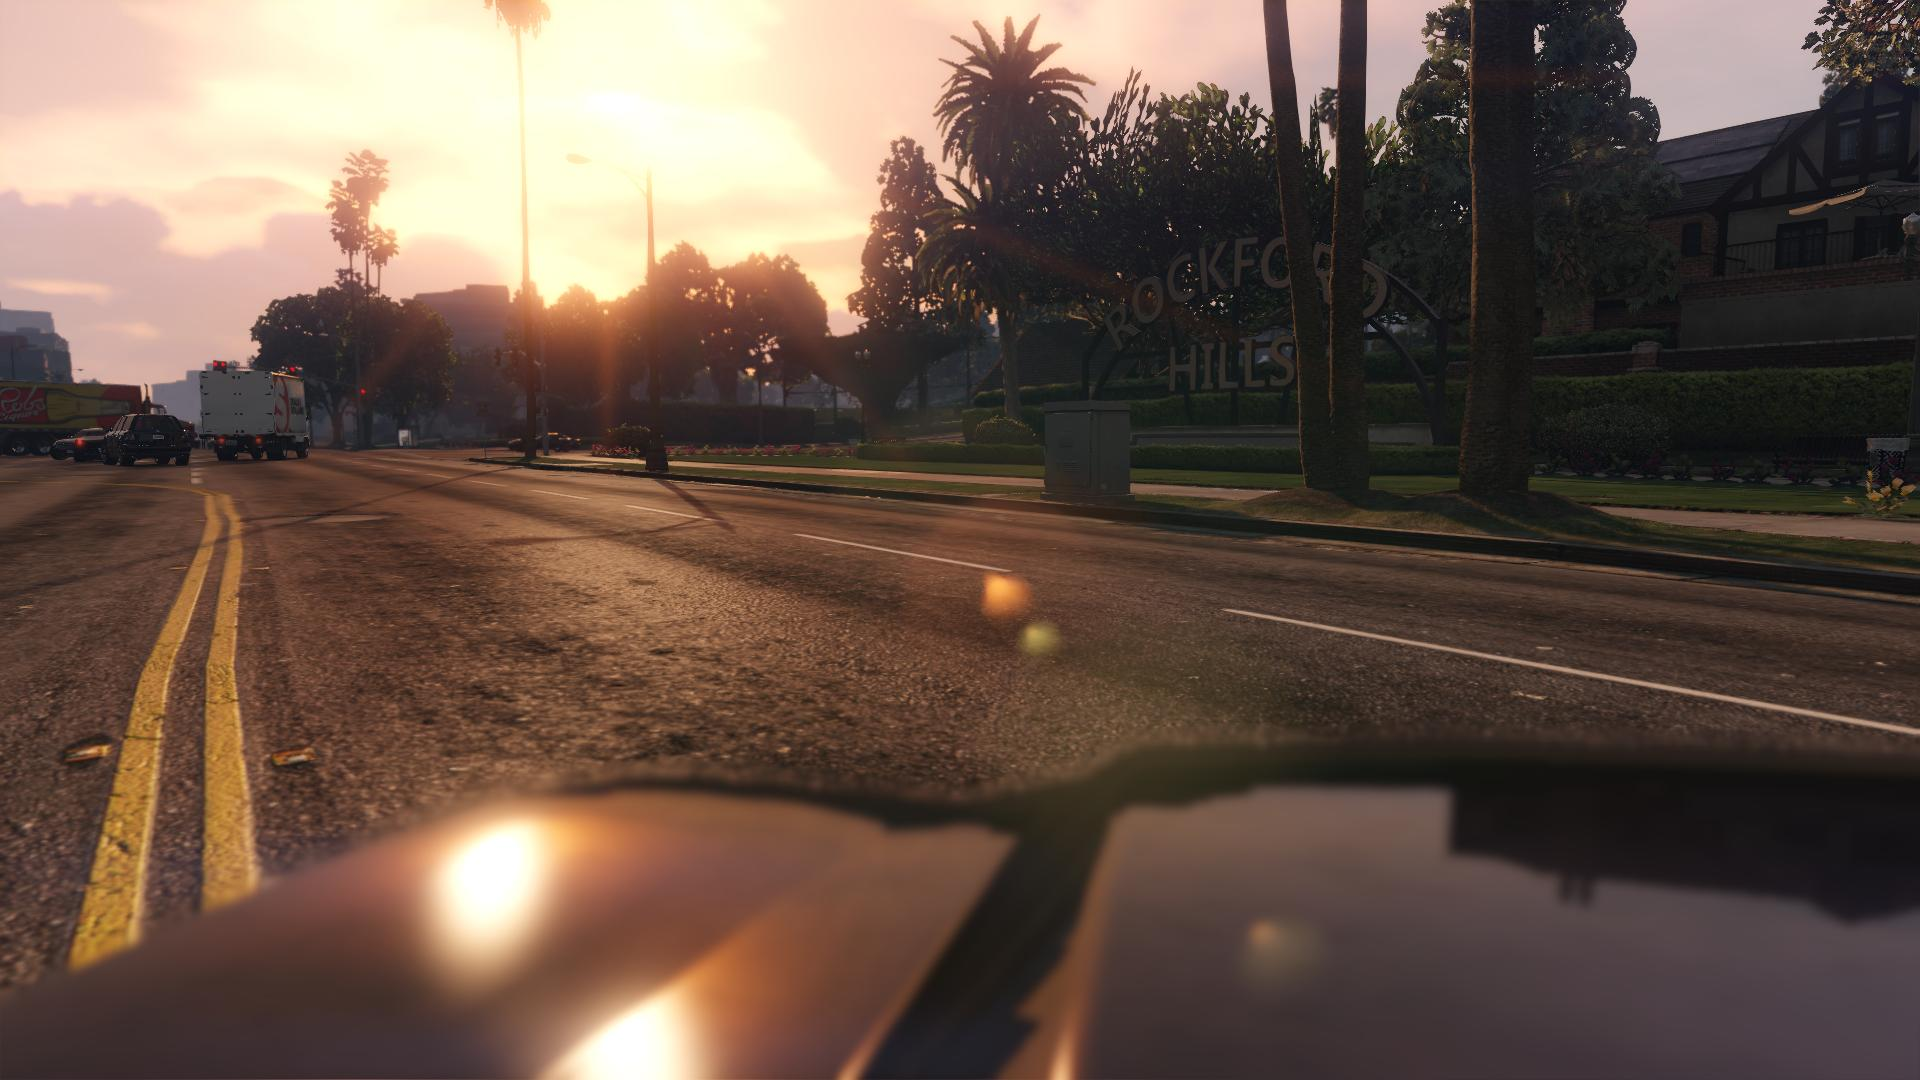
\includegraphics[width=0.5\linewidth]{Experiments/viper/011_01171}
				}
				\includegraphics[width=0.45\linewidth]{Experiments/viper/pdf/bird-0007}
				\caption{
					Left turn, reflections from sun
					\label{fig:viper-qualitative-sun-reflections}
				}
			\end{subfigure}%
			\\
			\begin{subfigure}[b]{\linewidth}
				\centering
				\raisebox{5mm}{
					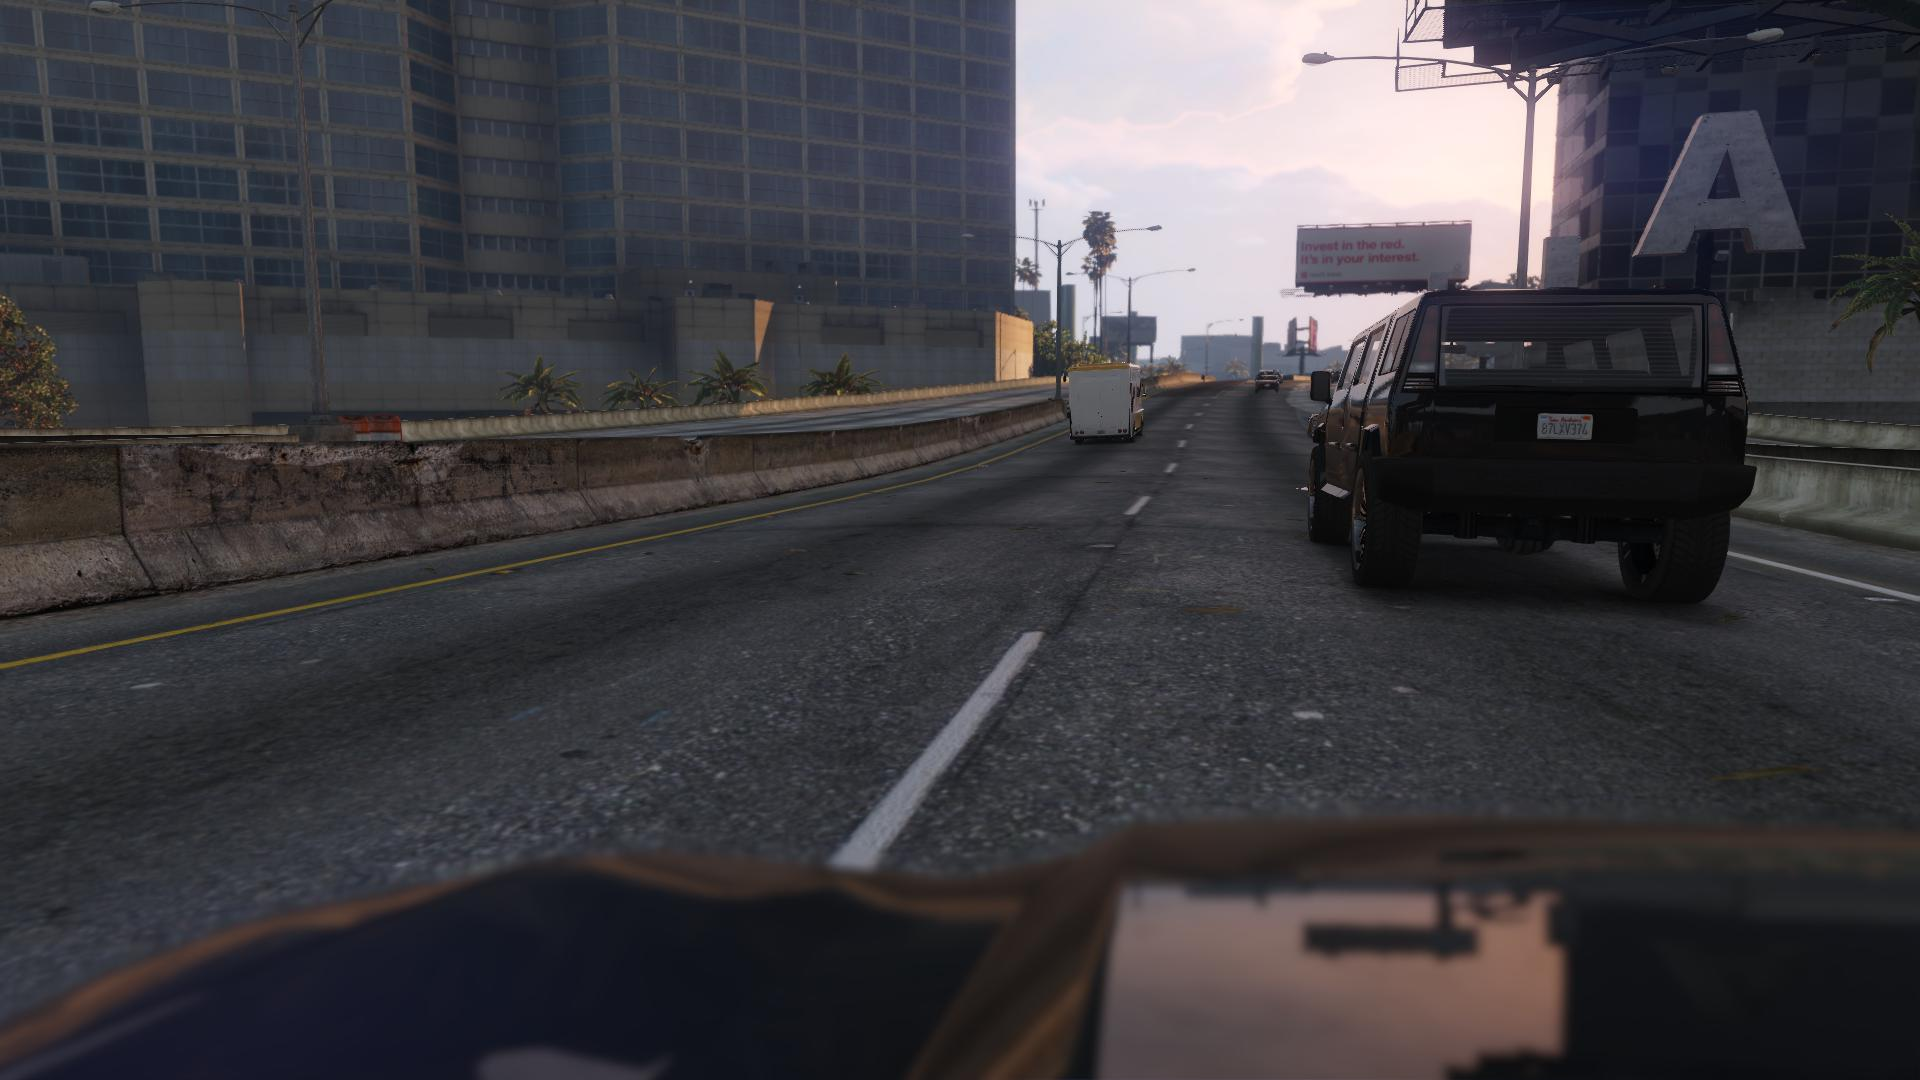
\includegraphics[width=0.5\linewidth]{Experiments/viper/016_00167}
				}
				\includegraphics[width=0.45\linewidth]{Experiments/viper/pdf/bird-0008}
				\caption{
					Passing maneuver on highway
					\label{fig:viper-qualitative-passing-maneuver}
				}
			\end{subfigure}%
			\\
			\begin{subfigure}[b]{\linewidth}
				\centering
				\raisebox{5mm}{
					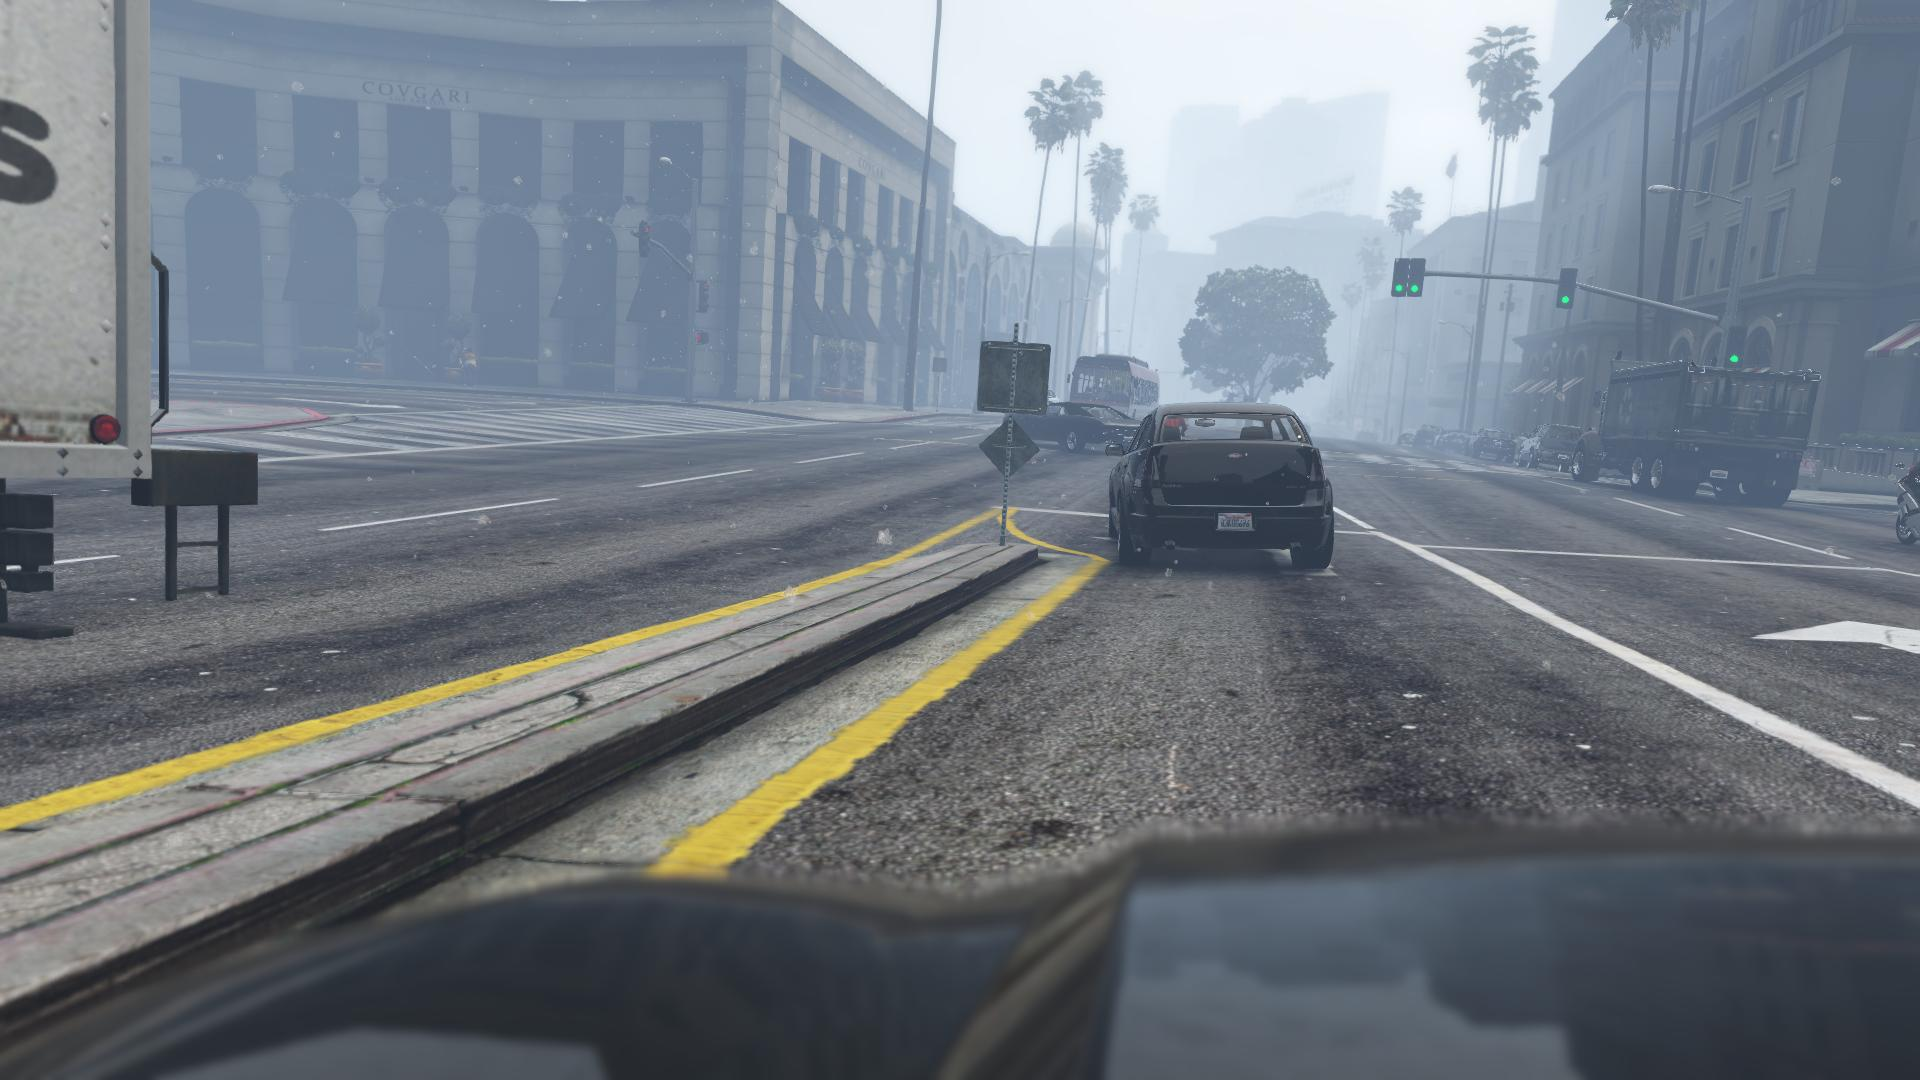
\includegraphics[width=0.5\linewidth]{Experiments/viper/021_00930}
				}
				\includegraphics[width=0.45\linewidth]{Experiments/viper/pdf/bird-0010}
				\caption{
					Left turn on crowded intersection, light snow and fog
					\label{fig:viper-qualitative-snow-crowded-intersection}
				}
			\end{subfigure}%
			\\
			\begin{subfigure}[b]{\linewidth}
				\centering
				\raisebox{5mm}{
					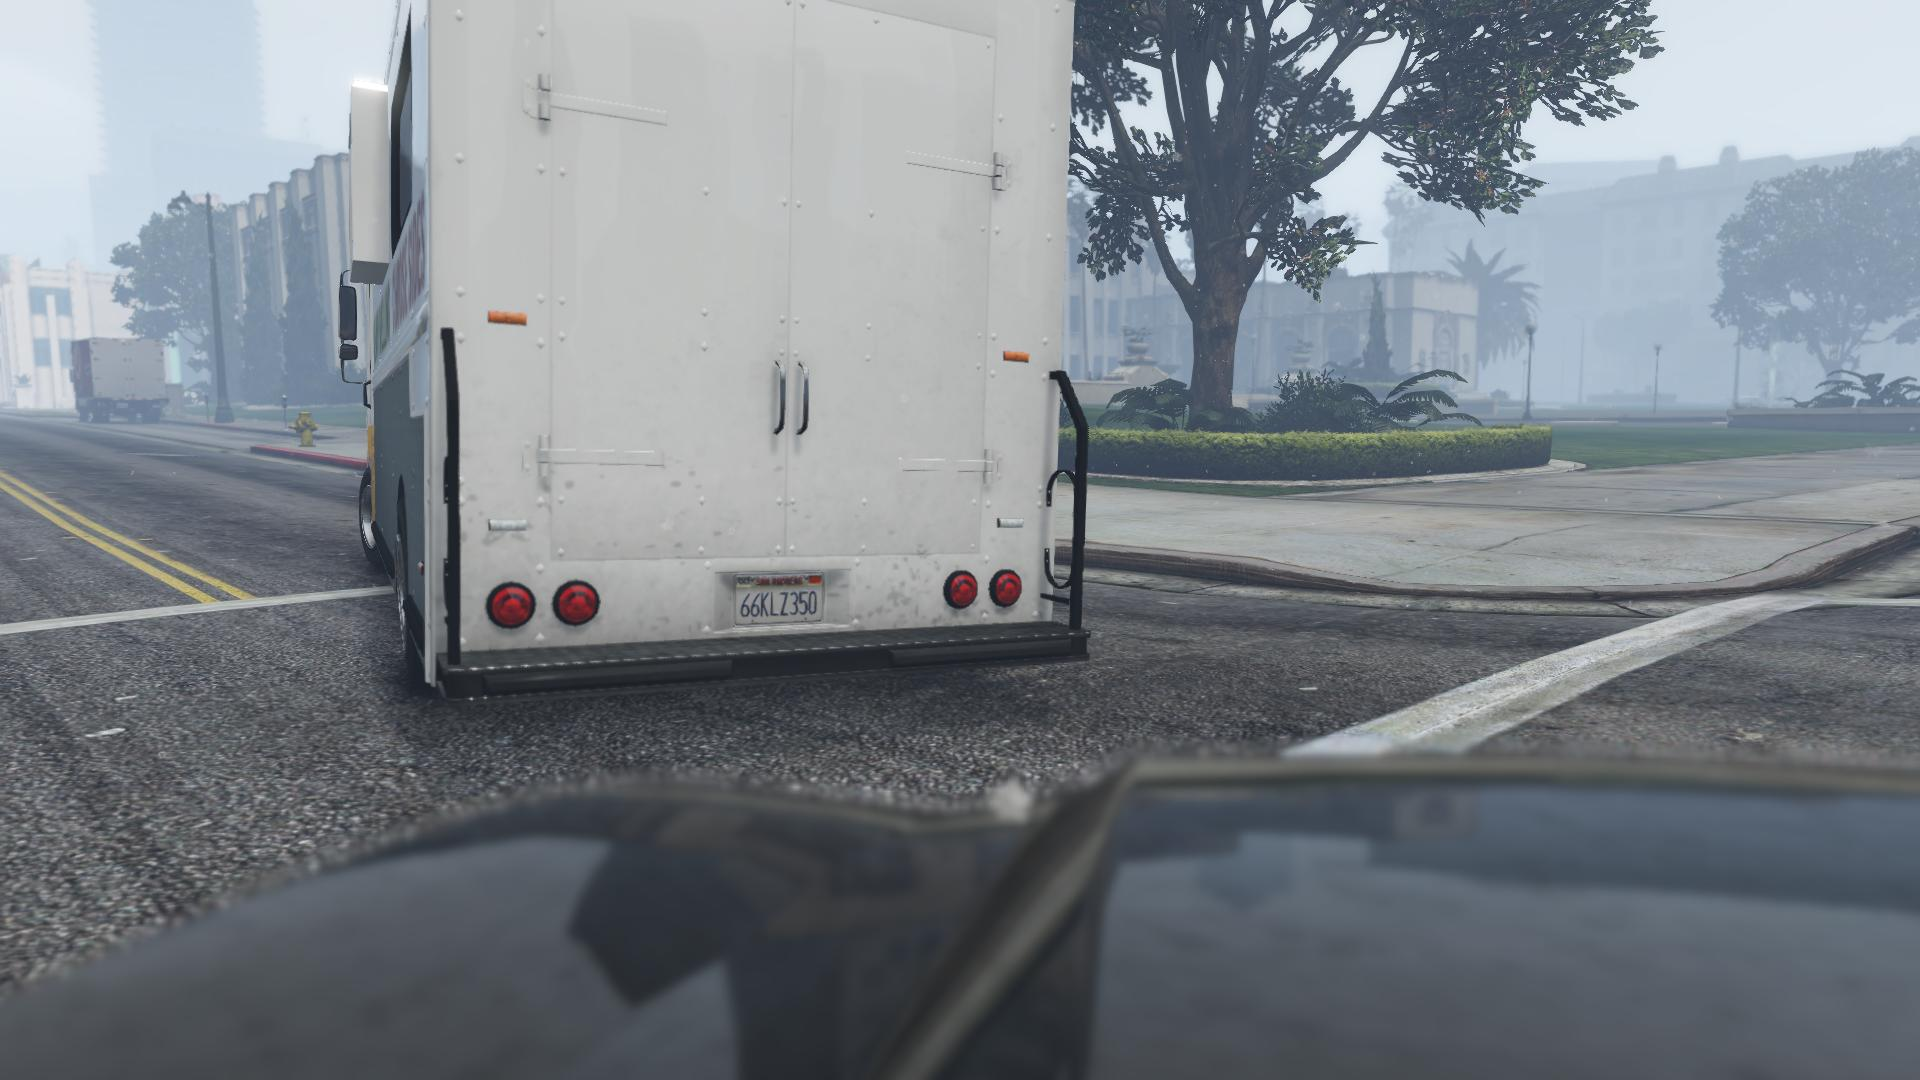
\includegraphics[width=0.5\linewidth]{Experiments/viper/027_00465}
				}				\includegraphics[width=0.45\linewidth]{Experiments/viper/pdf/bird-0012}
				\caption{
					Left turn on intersection following a truck in close proximity
					\label{fig:viper-qualitative-truck-left-turn-close}
				}
			\end{subfigure}%
			\caption[Qualitative results for motion estimation on VIPER]
					{Qualitative results for motion estimation on the VIPER test set.
					 Left column: An image from the video showing the scene type and motion scenario.
					 Right column: Bird's-eye view of the estimated and true camera motion.
					 The height dimension is omitted.
					 Each video is 100 frames long and a marker is shown for every 10th frame.
					 \label{fig:viper-qualitative-results-images-and-estimation}}
		\end{figure}
		
		
		\begin{figure}[h]
			\centering
			\begin{subfigure}[b]{\linewidth}
				\centering
				\raisebox{5mm}{
					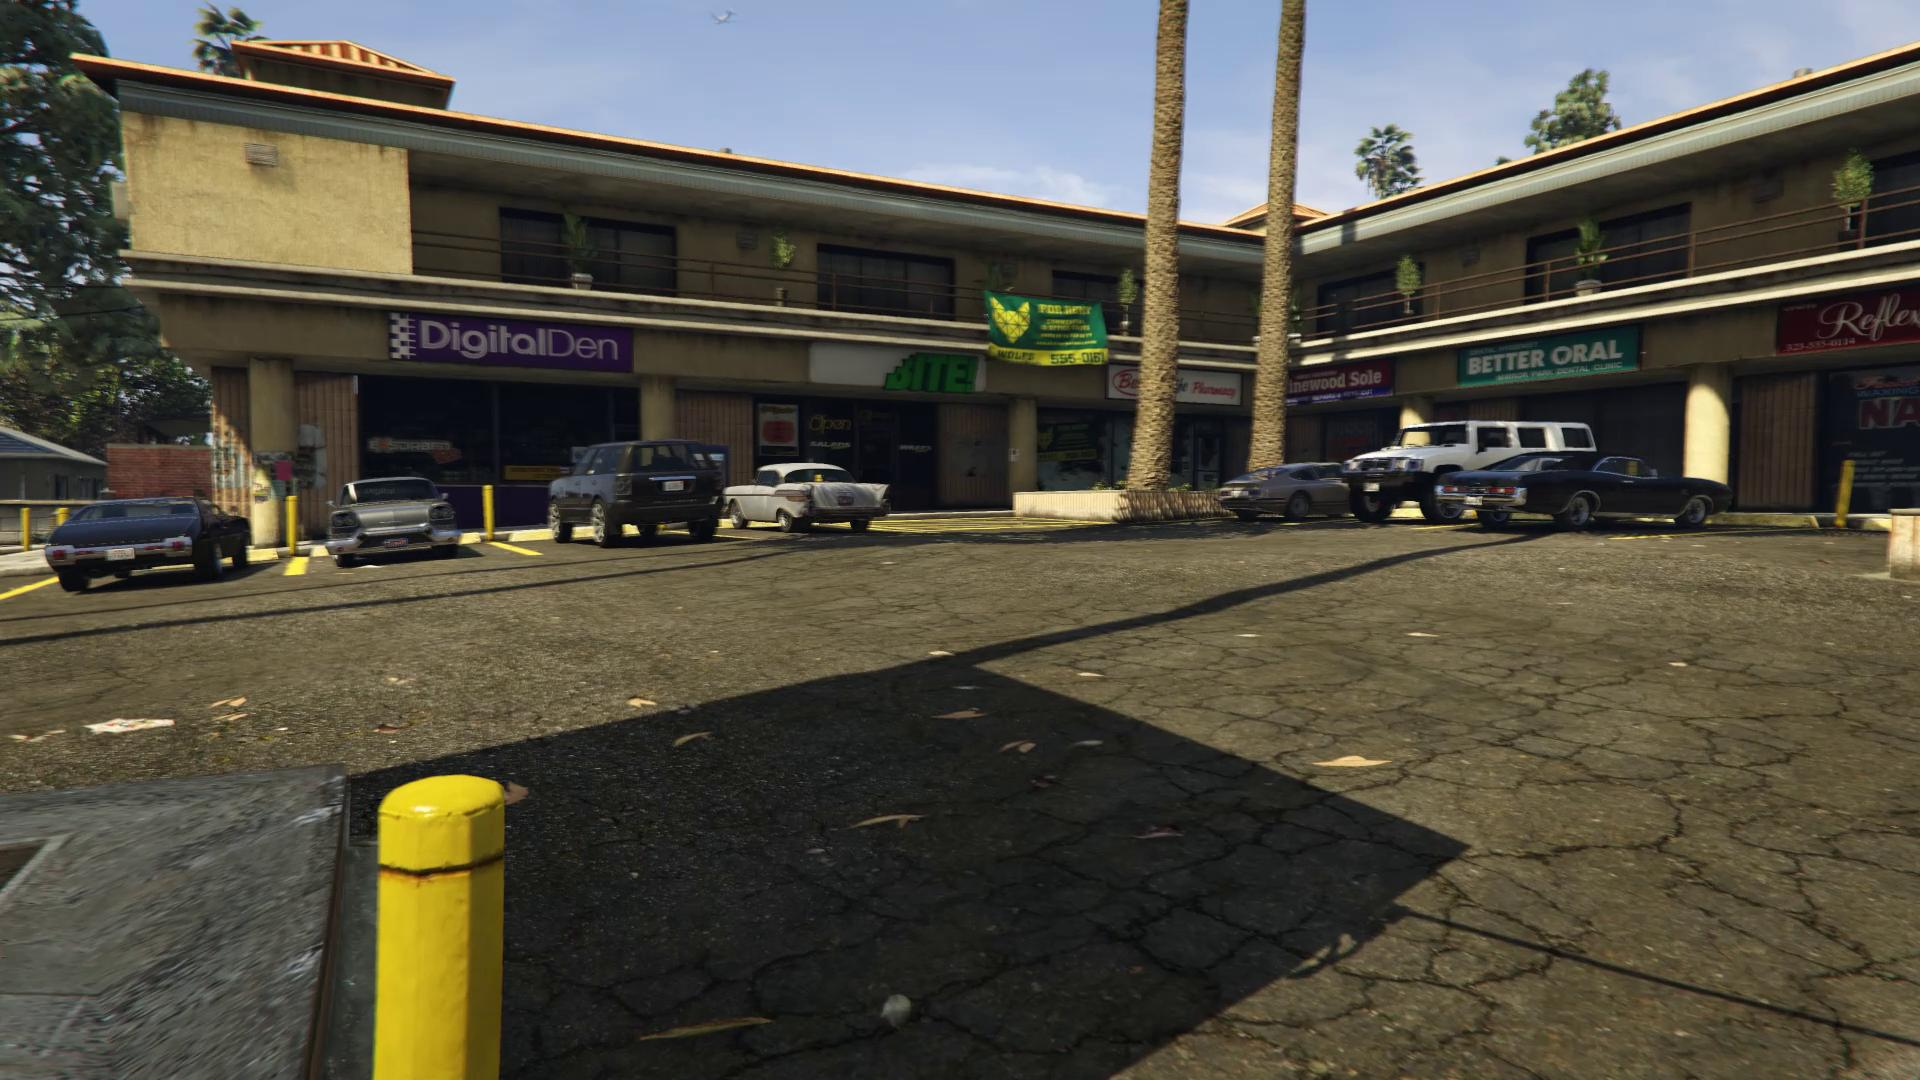
\includegraphics[width=0.5\linewidth]{Experiments/gta/2075}
				}
				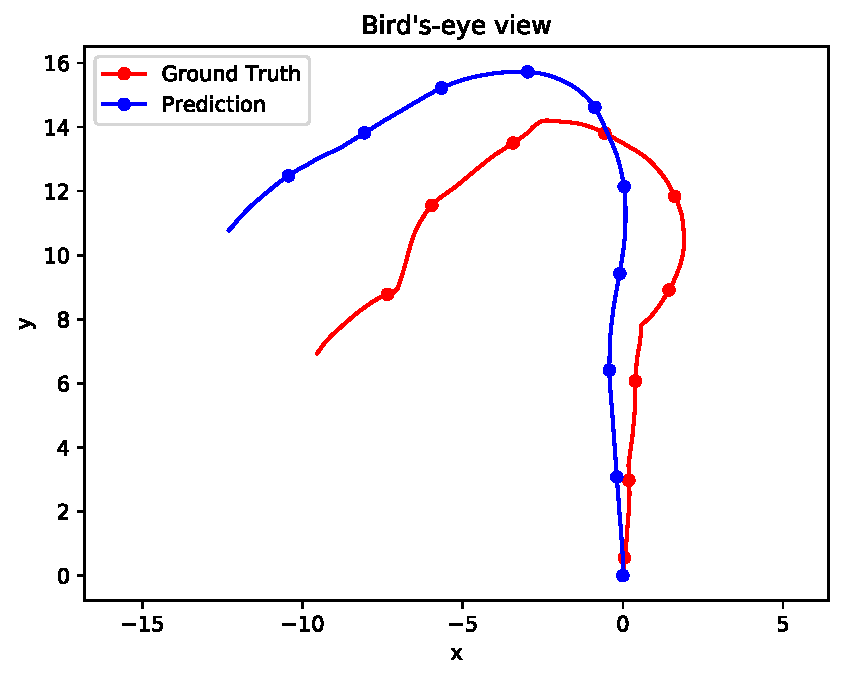
\includegraphics[width=0.45\linewidth]{Experiments/gta/pdf/bird-0001}
				\caption{
					Static scene, medium range
					\label{fig:gtav-qualitative-long-range-with-image}
				}
			\end{subfigure}%
			\\
			\begin{subfigure}[b]{\linewidth}
				\centering
				\raisebox{5mm}{
					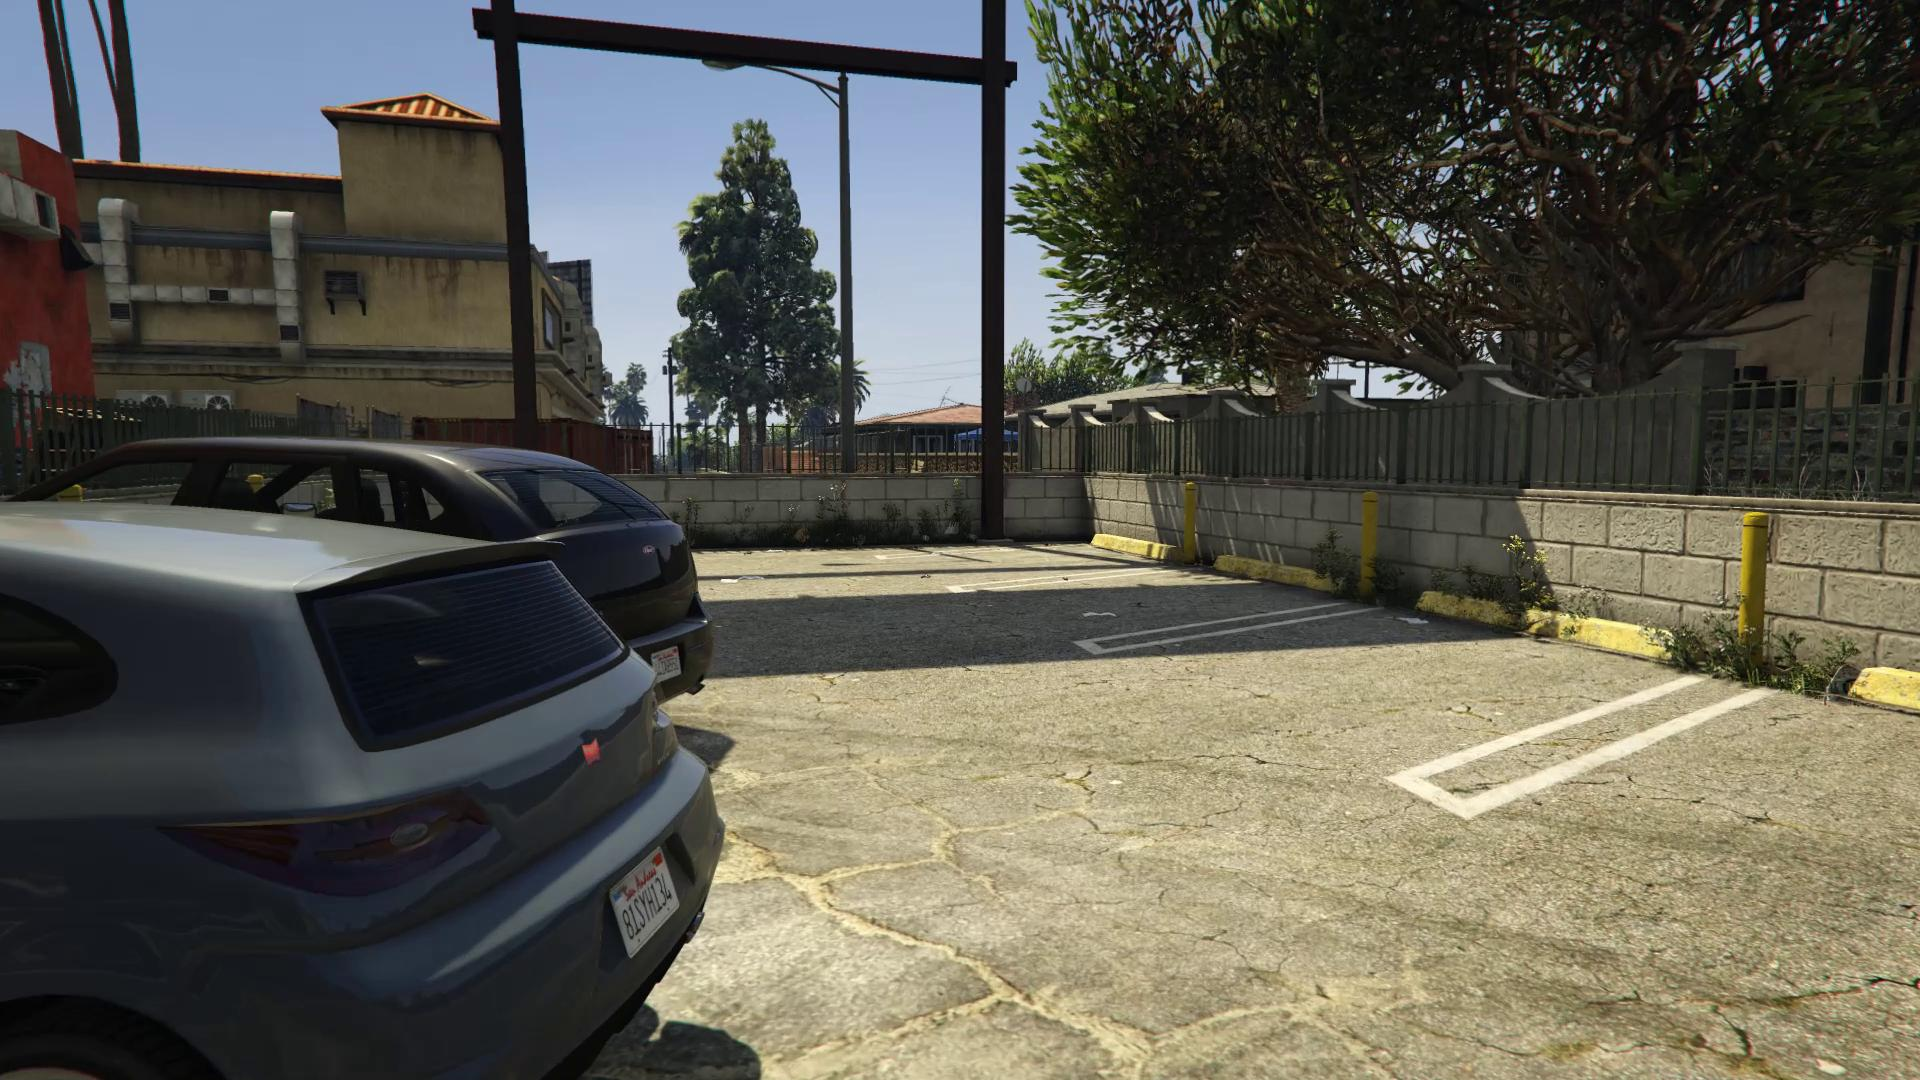
\includegraphics[width=0.5\linewidth]{Experiments/gta/87612}
				}
				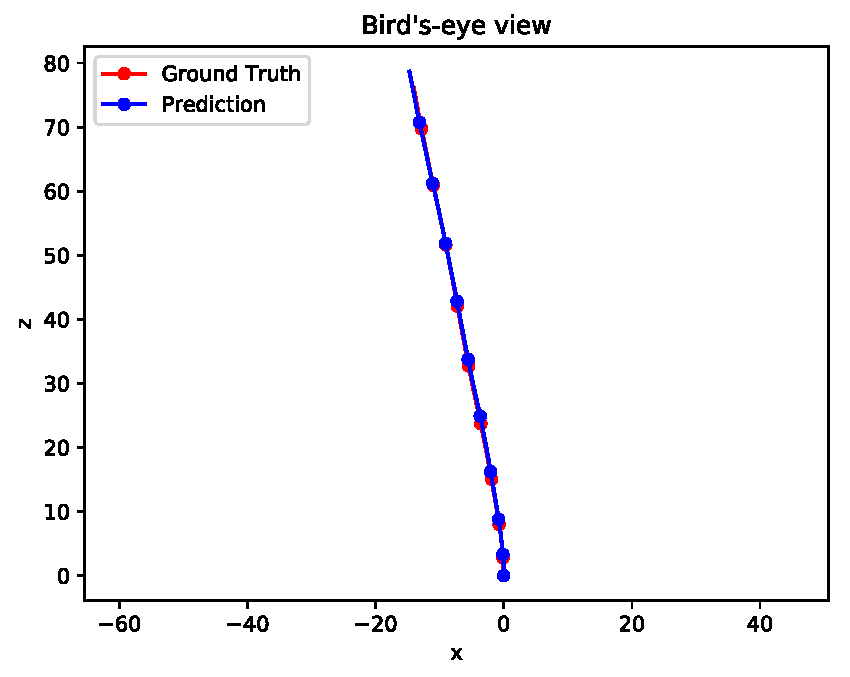
\includegraphics[width=0.45\linewidth]{Experiments/gta/pdf/bird-0011}
				\caption{
					Static scene, close range
					\label{fig:gtav-qualitative-close-range-with-image}
				}
			\end{subfigure}%
			\\
			\begin{subfigure}[b]{\linewidth}
				\centering
				\raisebox{5mm}{
					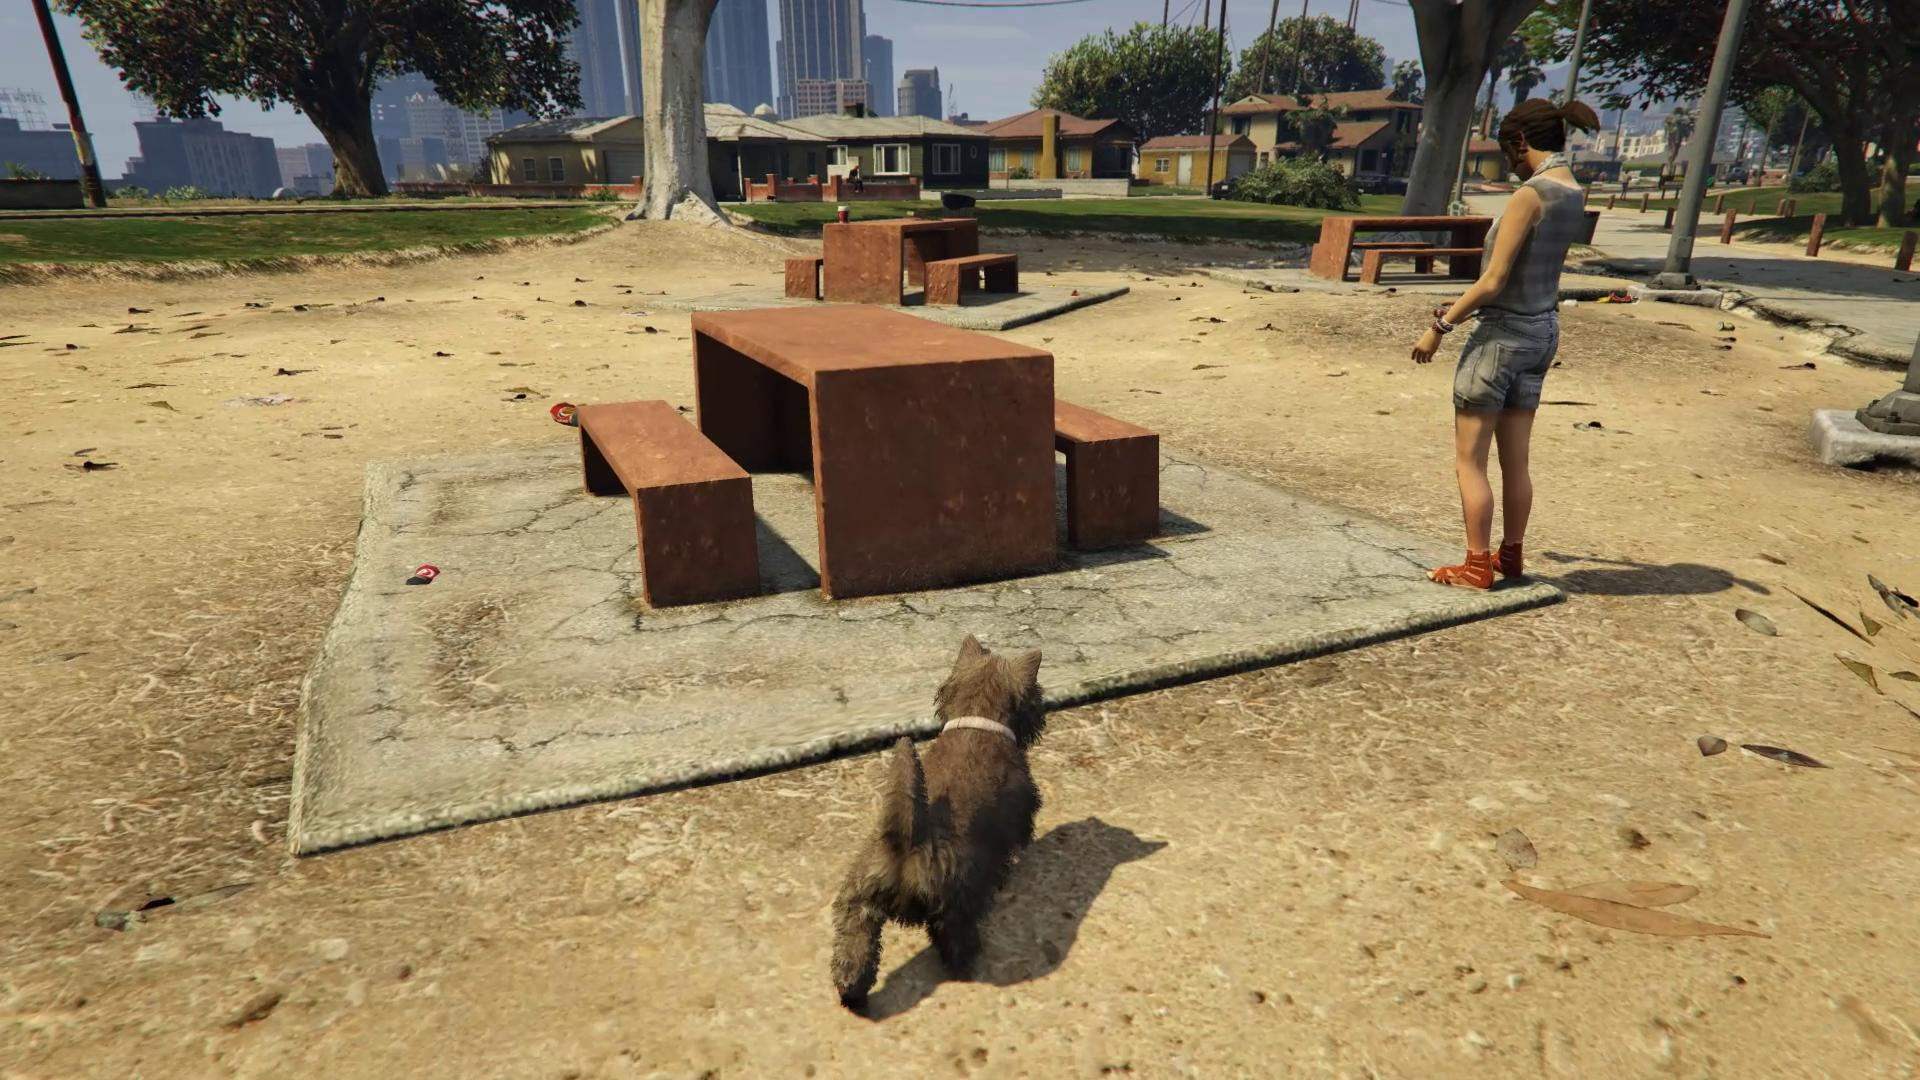
\includegraphics[width=0.5\linewidth]{Experiments/gta/375962}
				}
				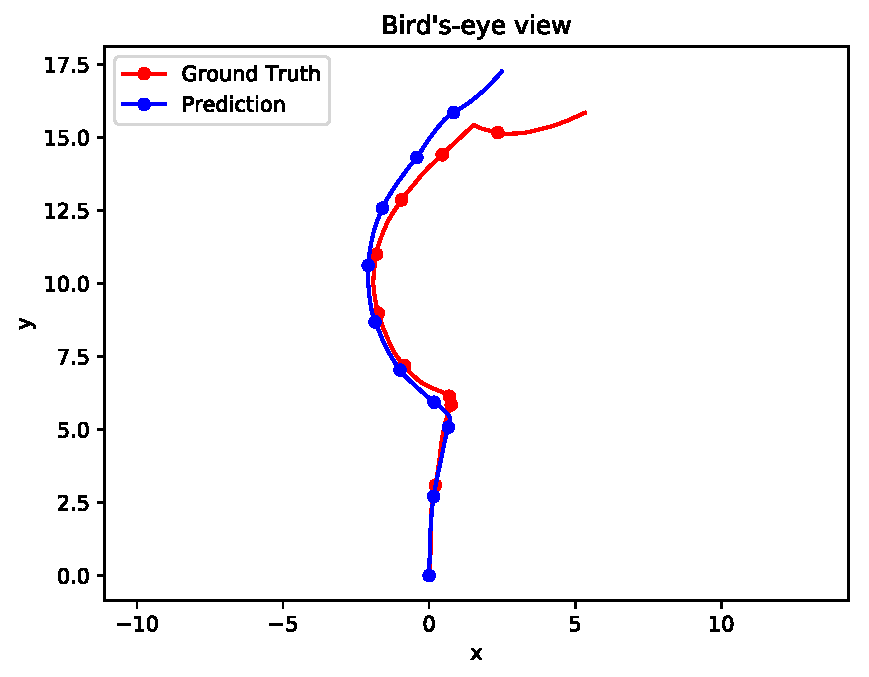
\includegraphics[width=0.45\linewidth]{Experiments/gta/pdf/bird-0005}
				\caption{
					Forward, stop, motion around fixed look-at point
					\label{fig:gtav-qualitative-look-at-fixed-with-image}
				}
			\end{subfigure}%
			\\
			\begin{subfigure}[b]{\linewidth}
				\centering
				\raisebox{5mm}{
					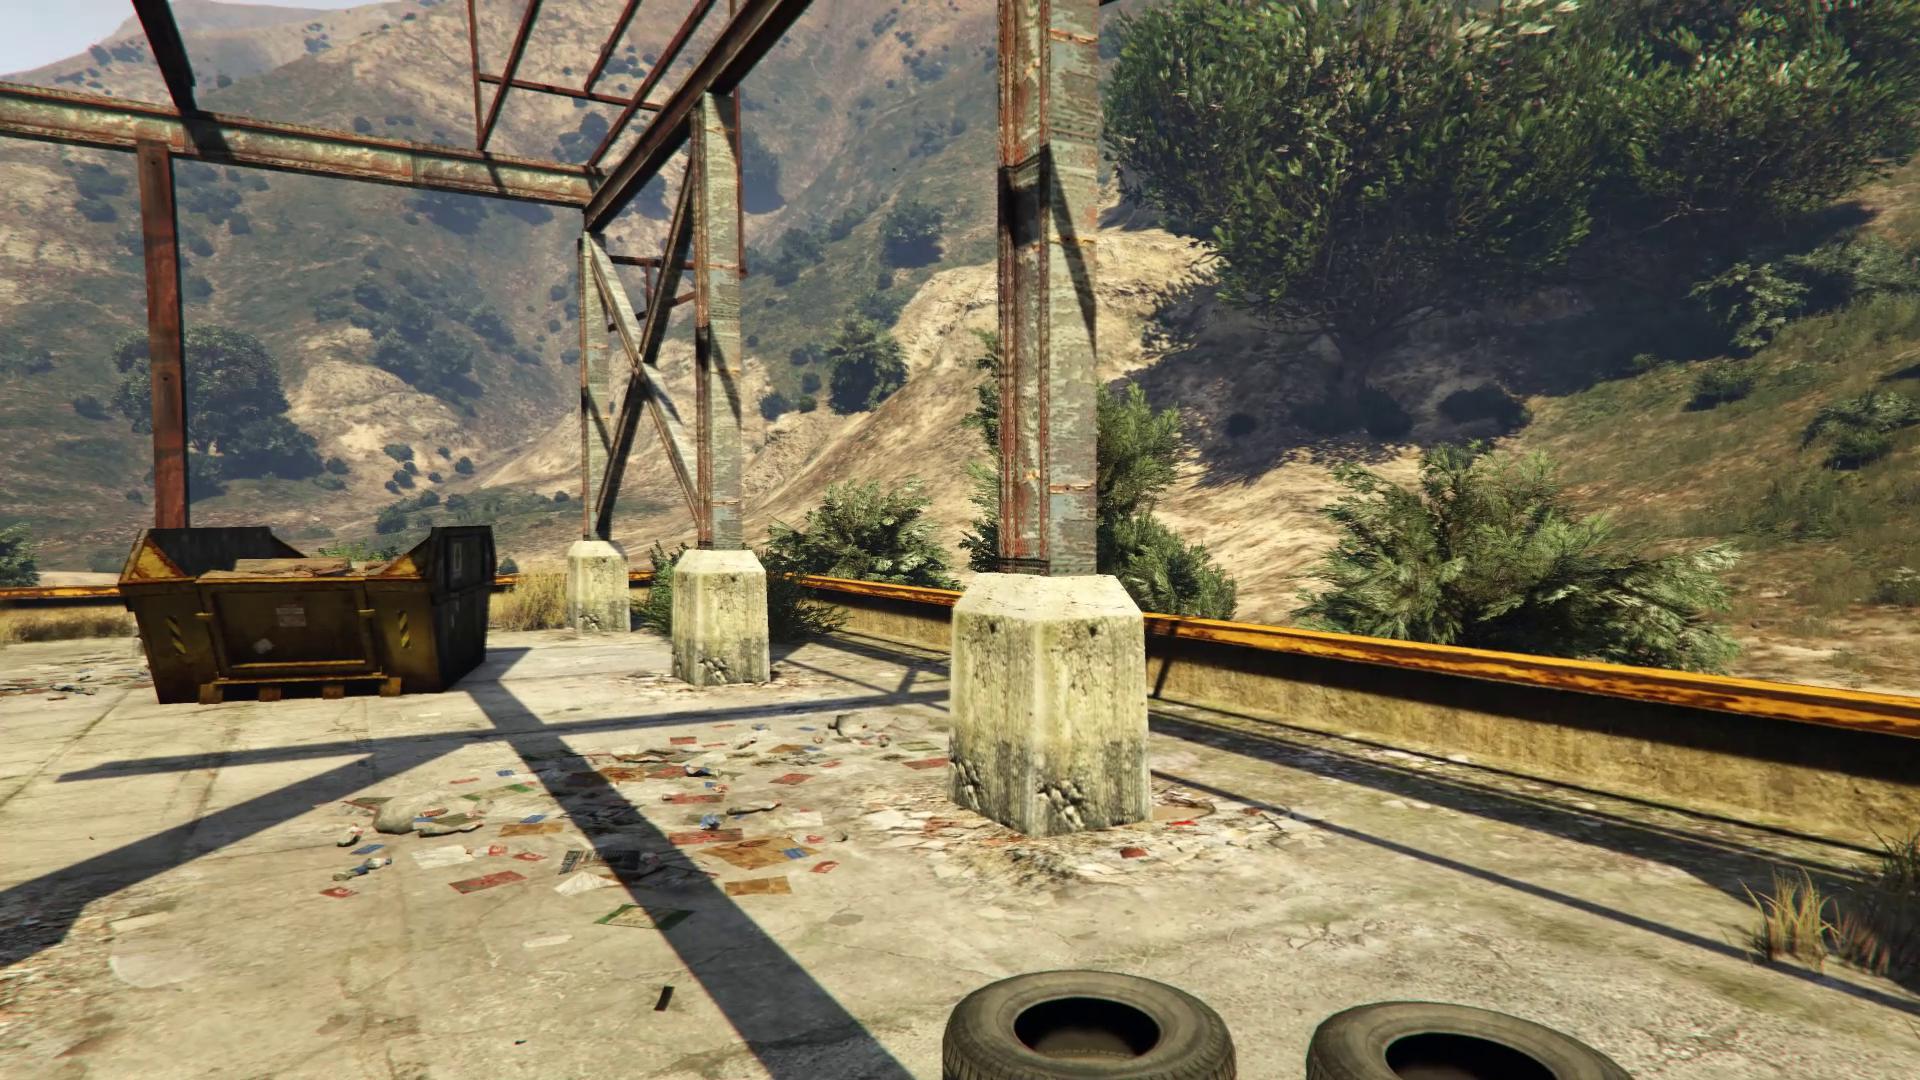
\includegraphics[width=0.5\linewidth]{Experiments/gta/15827}
				}
				\includegraphics[width=0.45\linewidth]{Experiments/gta/pdf/bird-0012}
				\caption{
					Forward, stop, $90^\circ$ turn, forward
					\label{fig:gtav-qualitative-sharp-turn-with-image}
				}
			\end{subfigure}%
			\caption[Qualitative results for motion estimation on GTA V - Part 1]
					{Qualitative results for motion estimation on the GTA V test set (part 1).
					 Left column: The first frame of the 200 frames long video.
					 Right column: Visualization of the estimated and true path from the bird's-eye perspective where the height dimension is omitted.
					 The plots show a marker for every 20th frame.
					 \label{fig:gtav-qualitative-results-images-and-translation}}
		\end{figure}
		
		
		\begin{figure}[h]
			\centering
			\begin{subfigure}[b]{\linewidth}
				\centering
				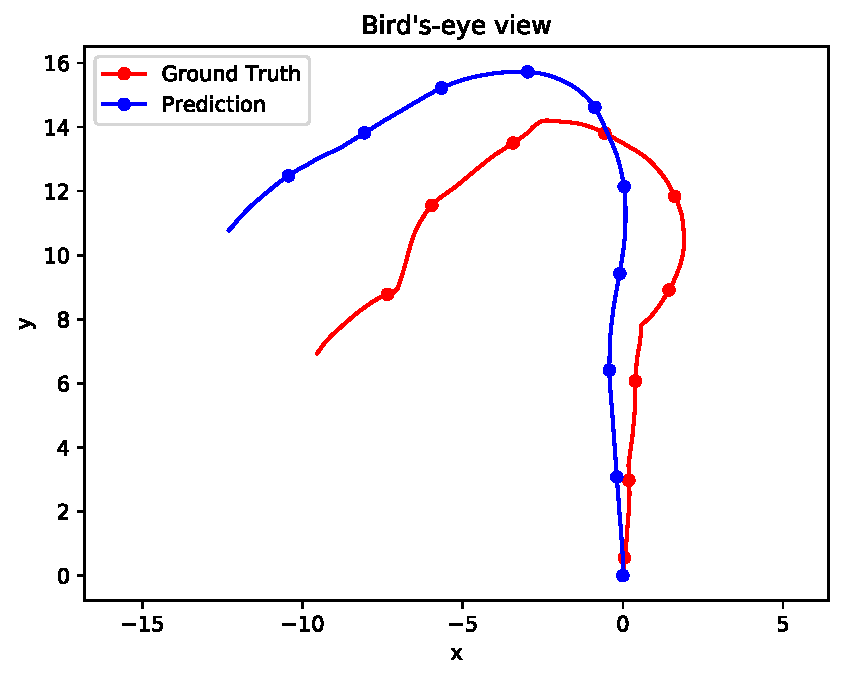
\includegraphics[width=0.45\linewidth]{Experiments/gta/pdf/bird-0001}
				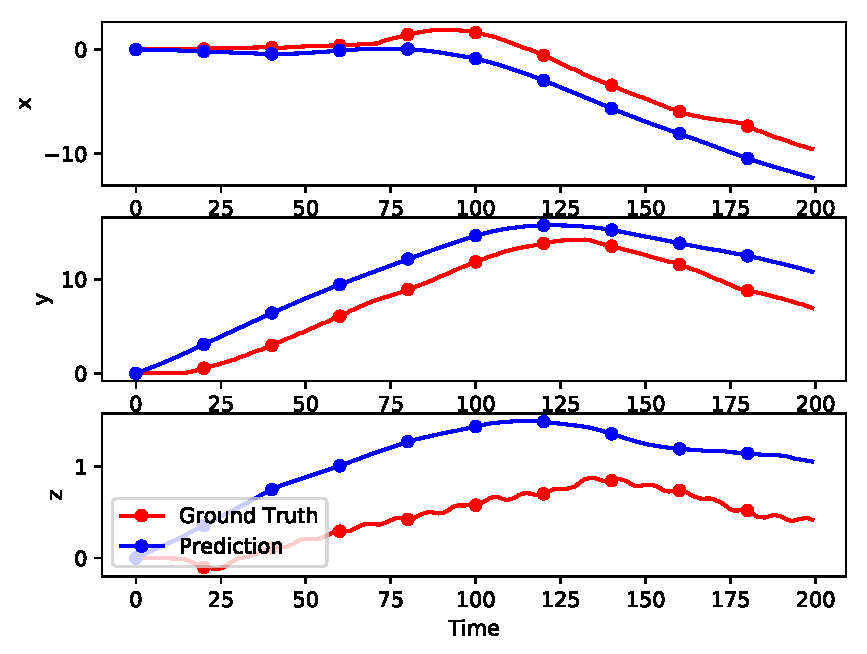
\includegraphics[width=0.45\linewidth]{Experiments/gta/pdf/b-0001}
				\caption{
					Static scene, medium range
					\label{fig:gtav-qualitative-long-range}
				}
			\end{subfigure}%
			\\
			\begin{subfigure}[b]{\linewidth}
				\centering
				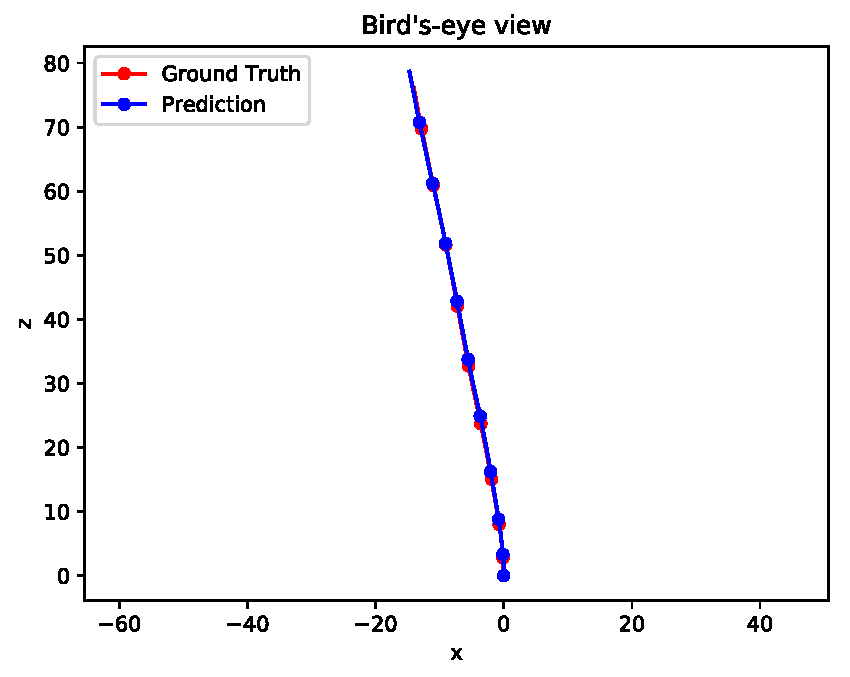
\includegraphics[width=0.45\linewidth]{Experiments/gta/pdf/bird-0011}
				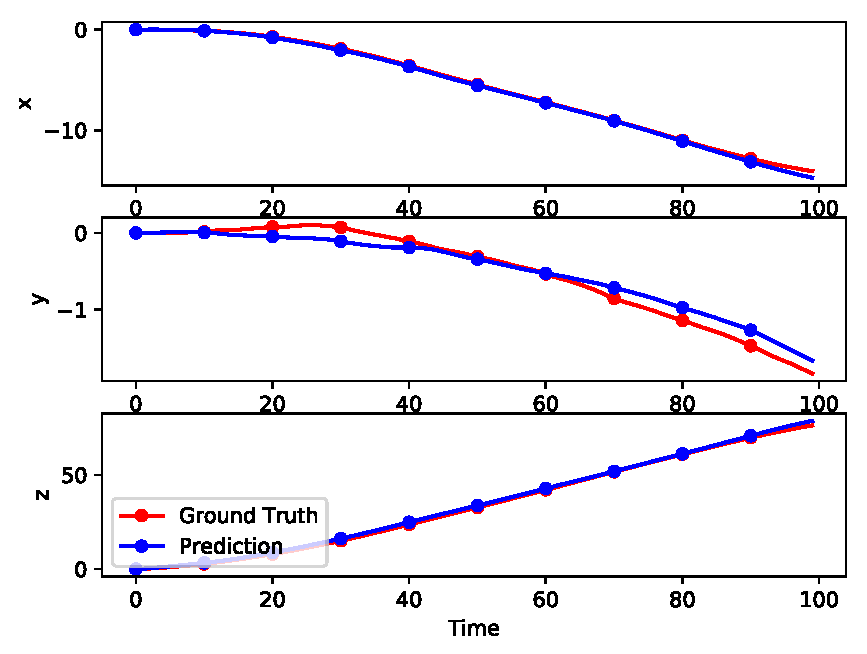
\includegraphics[width=0.45\linewidth]{Experiments/gta/pdf/b-0011}
				\caption{
					Static scene, close range
					\label{fig:gtav-qualitative-close-range}
				}
			\end{subfigure}%
			\\
			\begin{subfigure}[b]{\linewidth}
				\centering
				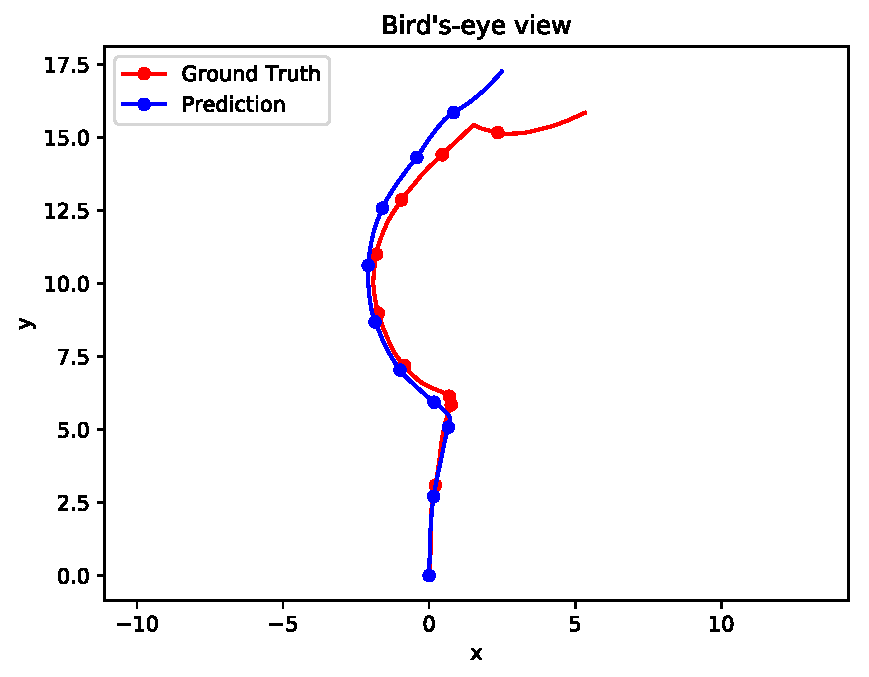
\includegraphics[width=0.45\linewidth]{Experiments/gta/pdf/bird-0005}
				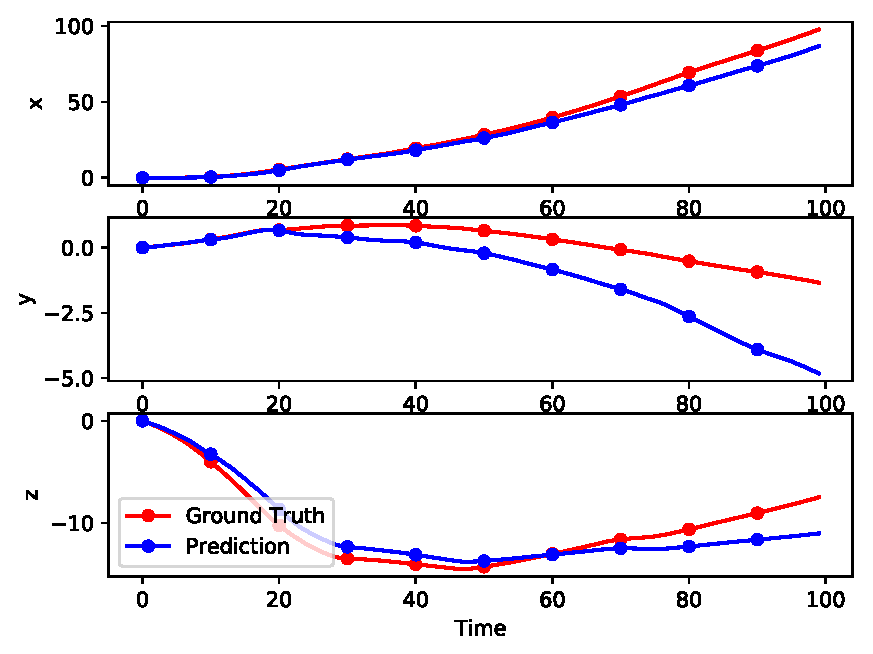
\includegraphics[width=0.45\linewidth]{Experiments/gta/pdf/b-0005}
				\caption{
					Forward, stop, motion around fixed look-at point
					\label{fig:gtav-qualitative-look-at-fixed}
				}
			\end{subfigure}%
			\\
			\begin{subfigure}[b]{\linewidth}
				\centering
				\includegraphics[width=0.45\linewidth]{Experiments/gta/pdf/bird-0012}
				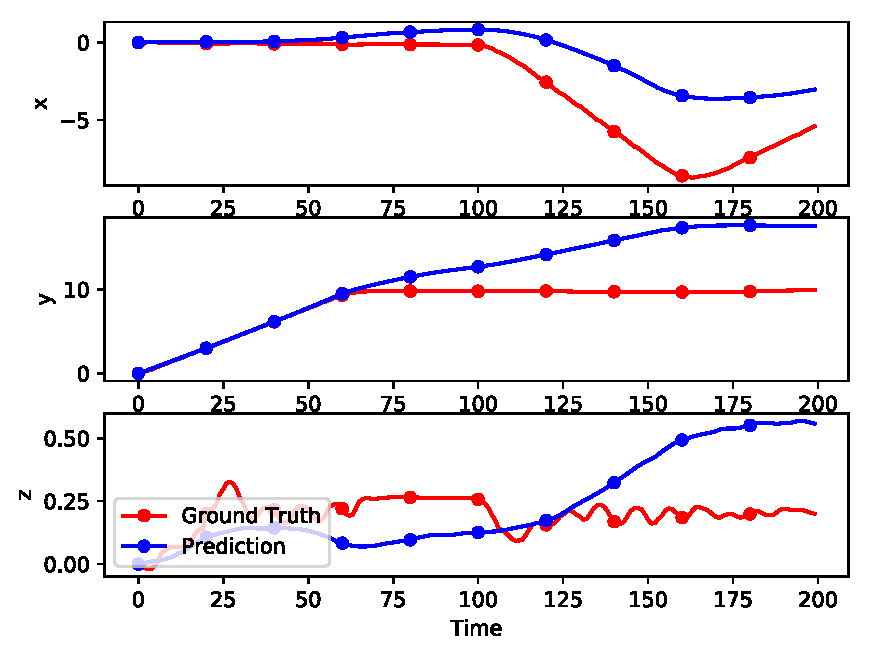
\includegraphics[width=0.45\linewidth]{Experiments/gta/pdf/b-0012}
				\caption{
					Forward, stop, $90^\circ$ turn, forward
					\label{fig:gtav-qualitative-sharp-turn}
				}
			\end{subfigure}%
			\caption[Qualitative results for motion estimation on GTA V - Part 2]
					{Qualitative results for motion estimation on the GTA V test set (part 2).
					 Left column: Visualization of the estimated and true path of the same videos from figure~\ref{fig:gtav-qualitative-results-images-and-translation}.
					 Right column: Plot of each coordinate axis of the translation.
					 The horizontal axis is the time (frame count).
					 The plots show a marker for every 20th frame.
					 \label{fig:gtav-qualitative-results-translation}}
		\end{figure}